\documentclass[12pt, a4paper]{article}

\usepackage[utf8]{inputenc}
\usepackage{amsmath, amssymb}
\usepackage{graphicx}
\usepackage{hyperref}
\usepackage{geometry}
\usepackage{booktabs}
\usepackage{listings}
\usepackage{xcolor}
\usepackage{tikz}
\usepackage{placeins}
\usepackage{float}
\usepackage{caption}
\usepackage{subcaption}
\usepackage{enumitem}
\usepackage{tabularx}

\usetikzlibrary{shapes.geometric, arrows, positioning, calc, fit, backgrounds, automata}

\geometry{margin=1in}

% Hyperref setup
\hypersetup{
    colorlinks=true,
    linkcolor=blue!70!black,
    citecolor=blue!70!black,
    urlcolor=blue!70!black
}

% Code snippet styling
\definecolor{codegreen}{rgb}{0,0.6,0}
\definecolor{codegray}{rgb}{0.5,0.5,0.5}
\definecolor{codepurple}{rgb}{0.58,0,0.82}
\definecolor{backcolour}{rgb}{0.96,0.96,0.94}
\definecolor{codeblue}{rgb}{0.13,0.13,1}

\lstdefinestyle{mystyle}{
    backgroundcolor=\color{backcolour},   
    commentstyle=\color{codegreen},
    keywordstyle=\color{magenta},
    numberstyle=\tiny\color{codegray},
    stringstyle=\color{codepurple},
    basicstyle=\ttfamily\footnotesize,
    breakatwhitespace=false,         
    breaklines=true,                 
    captionpos=b,                    
    keepspaces=true,                 
    numbers=left,                    
    numbersep=5pt,                  
    showspaces=false,                
    showstringspaces=false,
    showtabs=false,                  
    tabsize=2
}
\lstset{style=mystyle}

\begin{document}

% -------------------------------------------------------------
% TITLE PAGE
% -------------------------------------------------------------
\begin{titlepage}
    \centering
    
    
\includegraphics[width=0.91\textwidth]{Jadavpur_University_Logo.svg.png}\\[2 cm]

    {\huge \textbf{JADAVPUR UNIVERSITY}}\\[1.3cm]
    
    {\Large
    \textbf{Name:} Diptarko Bhattacharjee\\[0.65cm]
    \textbf{Roll:} 002410501013\\[0.65cm]
    \textbf{Class:} BCSE - UG 3 - Sem 1 - A1\\[0.65cm]
    \textbf{Subject:} Computer Networks Lab Assignment 3 Report\\
    }
    
\end{titlepage}

\newpage
\vspace*{-1cm}
\tableofcontents
\vspace*{-1cm}
\newpage


\title{Assignment 3: Design and Implement Medium Access Control Protocols (1-Persistent, Non-Persistent, $p$-Persistent CSMA, and CSMA/CD with Exponential Backoff)}
\author{Diptarko Bhattacharjee}
\date{}
\maketitle

% -------------------------------------------------------------
% SECTION 1: INTRODUCTION
% -------------------------------------------------------------
\section{Introduction}

In a computer network, whenever multiple communicating devices share a single physical transmission medium---such as a coaxial bus cable, a twisted-pair local area network, an optical link, or an open wireless radio channel---a fundamental coordination dilemma arises. If two or more stations attempt to transmit data frames across the shared physical channel simultaneously, their electrical or electromagnetic signals physically superimpose and corrupt one another. This catastrophic event is termed a \textbf{packet collision}, rendering the transmitted frames unintelligible to the intended receivers and destroying the channel's communication capacity.

To orchestrate orderly communication, prevent chaotic mutual interference, and maximize channel utilization, the Data Link Layer (OSI Layer 2) implements a specialized sub-layer known as the \textbf{Medium Access Control (MAC) Sublayer}. Medium Access Control protocols determine which station obtains the right to transmit over the shared broadcast medium at any given instant.

\subsection{Evolution from ALOHA to Carrier Sensing}
The earliest random access protocol, developed in 1970 at the University of Hawaii, was \textbf{Pure ALOHA}. Under Pure ALOHA, stations acted completely blindly: whenever a station had data to send, it transmitted immediately without assessing whether the channel was already occupied. Consequently, frames collided whenever another station began transmitting during a \textbf{vulnerability period} of twice the frame transmission time ($2 T_{trans}$). The maximum theoretical throughput efficiency of Pure ALOHA is fundamentally bounded by:
\begin{equation}
    S_{Pure\text{-}ALOHA} = G e^{-2G} \implies S_{max} = \frac{1}{2e} \approx 18.4\%
\end{equation}
where $G$ represents the offered channel traffic load. 

By introducing discrete, synchronized time slots, \textbf{Slotted ALOHA} halved the vulnerability period to $1 T_{trans}$, elevating maximum throughput to:
\begin{equation}
    S_{Slotted\text{-}ALOHA} = G e^{-G} \implies S_{max} = \frac{1}{e} \approx 36.8\%
\end{equation}
While Slotted ALOHA doubled the capacity of Pure ALOHA, over $63\%$ of the shared channel bandwidth remained squandered due to collisions and idle slots.

The breakthrough in random access protocols came with the introduction of \textbf{Carrier Sense Multiple Access (CSMA)}. Rather than transmitting blindly like ALOHA, CSMA enforces the intuitive golden rule of multi-party conversation: \textbf{``Listen Before Talk''} (\textit{Carrier Sensing}). Before injecting an electromagnetic or digital frame into the channel, a station must first sense the medium to ascertain whether another station is currently transmitting.
\begin{itemize}
    \item If the medium is sensed \textbf{BUSY}, the station defers its transmission to prevent destroying the ongoing frame.
    \item If the medium is sensed \textbf{IDLE}, the station may initiate its transmission according to a predefined persistence algorithm.
\end{itemize}

\subsection{Assignment Objectives}
The primary objective of this laboratory assignment is to design, implement, and rigorously benchmark the family of Carrier Sense Multiple Access protocols within a distributed client-server architecture using POSIX UDP Socket Programming in C++. Specifically, this project entails:
\begin{enumerate}
    \item \textbf{Emulating a Shared Transmission Medium:} Engineering a standalone Channel Coordinator process (\texttt{channel.cpp}) that models the state of the shared physical ether as either \texttt{IDLE}, \texttt{BUSY}, or \texttt{COLLISION}, accurately simulating transmission windows, concurrency overlaps, and channel noise (packet loss and bit corruption).
    \item \textbf{Implementing Independent Station Processes:} Engineering independent, multi-process network client stations (\texttt{station.cpp}) capable of dynamically executing four distinct Medium Access Control strategies:
    \begin{itemize}
        \item \textbf{1-Persistent CSMA:} Continuously monitors the channel and transmits immediately upon the channel becoming idle.
        \item \textbf{Non-Persistent CSMA:} If the channel is sensed busy, halts carrier sensing and defers for a randomized backoff interval before re-probing the medium.
        \item \textbf{$p$-Persistent CSMA:} Implemented over a slotted medium; upon sensing an idle channel, transmits with probability $p$ or defers to the subsequent slot with probability $(1-p)$.
        \item \textbf{CSMA/CD (Carrier Sense Multiple Access with Collision Detection):} Emulates IEEE 802.3 Ethernet behavior by enforcing ``Listen While Transmit''. Upon detecting concurrent overlapping transmissions, it immediately aborts the transmission window, broadcasts an explicit collision indication (jam signal), and executes the \textbf{Truncated Binary Exponential Backoff (BEB)} algorithm.
    \end{itemize}
    \item \textbf{Empirical and Theoretical Benchmarking:} Analyzing how the number of contending stations ($N$) and the persistence parameter ($p$) govern the number of collisions, average transmission delay, and aggregate channel throughput, comparing our empirical socket results against classical mathematical models.
\end{enumerate}


% -------------------------------------------------------------
% SECTION 2: THEORETICAL ANALYSIS \& MATHEMATICAL MODELING
% -------------------------------------------------------------
\section{Theoretical Analysis \& Mathematical Modeling}

To appreciate the architectural differences among the four simulated protocols, we must formalize their mathematical operating principles, vulnerability windows, and throughput equations.

\subsection{Vulnerability Period and Propagation Delay ($\tau$)}
A common misconception is that Carrier Sensing completely eradicates collisions. In physical reality, signals propagate across a medium at a finite speed (approximately $2 \times 10^8 \text{ m/s}$ in copper and optical fiber, or $3 \times 10^8 \text{ m/s}$ in vacuum). 

Let $\tau = T_p$ denote the maximum end-to-end \textbf{propagation delay} across the shared medium. If Station A begins transmitting at time $t = 0$, the electrical wavefront does not reach Station B at the opposite end of the wire until time $t = \tau$. If Station B senses the channel at time $t = \tau - \epsilon$ (where $\epsilon > 0$), Station B will detect an \textbf{IDLE} channel, conclude that no one is transmitting, and begin its own transmission. Moments later, the signals collide on the wire. Thus, the \textbf{vulnerability period} of standard CSMA is equal to the propagation delay:
\begin{equation}
    T_{vuln} = \tau = T_p
\end{equation}
The normalized propagation delay is defined as the dimensionless parameter:
\begin{equation}
    a = \frac{\tau}{T_{trans}} = \frac{T_p}{T_{trans}}
\end{equation}
where $T_{trans}$ is the frame transmission time ($T_{trans} = \frac{L}{R}$, frame length $L$ divided by channel bit rate $R$). For CSMA to perform efficiently, $a$ must be significantly less than 1 ($a \ll 1$). If $a \ge 1$, the propagation delay exceeds the packet duration, and CSMA degrades to the performance of Pure ALOHA.

\subsection{1-Persistent CSMA}
Under 1-Persistent CSMA, when a station has a frame to send:
\begin{enumerate}
    \item It continuously senses the channel.
    \item If the channel is sensed \textbf{BUSY}, it persists in listening until the medium becomes \textbf{IDLE}.
    \item The very instant the channel becomes idle, the station transmits its frame with a probability of $1$ (hence ``1-persistent'').
\end{enumerate}

\subsubsection{Theoretical Throughput Formula}
According to the classical analysis by Kleinrock and Tobagi (1975), the normalized throughput $S$ as a function of the offered traffic load $G$ is given by:
\begin{equation}
    S_{\text{1-Pers}} = \frac{G \left[ 1 + G + a G \left(1 + G + \frac{a G}{2}\right) \right] e^{-G(1 + 2a)}}{G(1 + 2a) - (1 - e^{-a G}) + (1 + a G) e^{-G(1 + a)}}
\end{equation}

\subsubsection{Vulnerability: The Collision Avalanche}
While 1-Persistent CSMA minimizes channel idleness by transmitting immediately when the wire becomes free, it suffers from a catastrophic flaw under medium-to-heavy traffic loads. If Station A is transmitting, other stations (say B, C, and D) that generate packets during Station A's transmission will all sense the wire to be busy. Under 1-persistent rules, all of them wait synchronously, listening to the wire. The instant Station A finishes and the channel becomes idle, Stations B, C, and D all transmit simultaneously. A collision is $100\%$ guaranteed. This triggers a destructive \textbf{collision avalanche}, driving channel throughput towards zero as the number of contending stations increases.

\subsection{Non-Persistent CSMA}
Non-Persistent CSMA was engineered specifically to prevent the synchronous collision avalanche of 1-persistent CSMA. Its operating rules are:
\begin{enumerate}
    \item Sense the channel.
    \item If the channel is \textbf{IDLE}, transmit the frame immediately.
    \item If the channel is \textbf{BUSY}, do \textit{not} continually monitor the wire. Instead, immediately abort sensing, pick a randomized backoff interval drawn from a random distribution, and enter a dormant sleep state.
    \item Upon the expiration of the backoff timer, re-sense the channel and repeat the algorithm.
\end{enumerate}

\subsubsection{Theoretical Throughput Formula}
The normalized throughput of Non-Persistent CSMA is mathematically modeled as:
\begin{equation}
    S_{\text{Non-Pers}} = \frac{G e^{-a G}}{G (1 + 2a) + e^{-a G}}
\end{equation}

\subsubsection{Tradeoff: Idleness vs. Collision Avoidance}
By forcing contending stations to sleep for independent random durations when the channel is busy, Non-Persistent CSMA successfully desynchronizes contending stations. When the current transmission finishes, the channel remains clear because competing stations are still sleeping. As a result, Non-Persistent CSMA achieves a vastly superior peak throughput ($S \approx 0.81$ when $a = 0.01$) compared to 1-Persistent CSMA ($S \approx 0.53$).

However, the cost of this collision avoidance is \textbf{channel underutilization at low traffic loads}. When traffic is light, the channel may sit completely empty while the only station with ready data is idling through a random backoff timer, thereby introducing unnecessary transmission latency.

\subsection{$p$-Persistent CSMA}
$p$-Persistent CSMA is an elegant hybrid protocol designed for slotted channels that strikes a mathematical balance between the aggressiveness of 1-Persistent CSMA and the conservatism of Non-Persistent CSMA. The time axis is divided into discrete slots equal to the maximum one-way propagation delay $\tau$.

When a station has a frame ready to transmit:
\begin{enumerate}
    \item It continuously senses the channel.
    \item If the channel is \textbf{BUSY}, it persists in sensing until the channel becomes \textbf{IDLE}.
    \item When the channel becomes \textbf{IDLE}, the station initiates a \textbf{Bernoulli trial} using a predefined probability parameter $p \in (0, 1]$:
    \begin{itemize}
        \item With probability $p$, it transmits the frame immediately.
        \item With probability $(1 - p)$, it defers transmission by exactly one time slot ($\tau$) and senses the channel again at the slot boundary.
    \end{itemize}
    \item At the next slot:
    \begin{itemize}
        \item If the channel is still \textbf{IDLE}, it repeats the Bernoulli trial (transmits with probability $p$, defers with probability $1-p$).
        \item If the channel has become \textbf{BUSY} (because another station began transmitting), it recognizes that it lost the contention, treats it as a collision, and initiates a random backoff procedure.
    \end{itemize}
\end{enumerate}

\subsubsection{Mathematical Derivation of Optimal $p$}
Suppose $N$ contending stations have packets queued when the channel becomes idle. The number of stations that transmit in the initial slot follows a Binomial distribution:
\begin{equation}
    P(k \text{ stations transmit}) = \binom{N}{k} p^k (1 - p)^{N - k}
\end{equation}
For a transmission to succeed without collision, \textit{exactly one} station must transmit ($k = 1$):
\begin{equation}
    P_{\text{success}} = P(k = 1) = N p (1 - p)^{N - 1}
\end{equation}
The probability that no station transmits, leaving the slot idle, is:
\begin{equation}
    P_{\text{idle}} = P(k = 0) = (1 - p)^N
\end{equation}
And the probability of a collision is:
\begin{equation}
    P_{\text{collision}} = 1 - P_{\text{success}} - P_{\text{idle}} = 1 - N p (1 - p)^{N - 1} - (1 - p)^N
\end{equation}

To maximize the probability of a successful transmission $P_{\text{success}}$, we differentiate with respect to $p$ and set the derivative to zero:
\begin{align}
    \frac{d}{dp} \left[ N p (1 - p)^{N - 1} \right] &= N (1 - p)^{N - 1} - N(N - 1) p (1 - p)^{N - 2} = 0 \\
    (1 - p) - (N - 1) p &= 0 \implies 1 - N p = 0 \\
    p^* &= \frac{1}{N}
\end{align}
Thus, the mathematically optimal persistence parameter is inversely proportional to the number of contending stations: $p^* = \frac{1}{N}$.
\begin{itemize}
    \item If $p > \frac{1}{N}$, too many stations transmit simultaneously, driving $P_{\text{collision}} \to 1$ and collapsing into 1-persistent failure.
    \item If $p \ll \frac{1}{N}$, no station transmits, driving $P_{\text{idle}} \to 1$. Dozens of consecutive slots are wasted in silence, causing transmission delay to explode.
\end{itemize}

\subsection{CSMA/CD (IEEE 802.3 Ethernet)}
In standard CSMA (1-Persistent, Non-Persistent, $p$-Persistent), once a station initiates transmission, it blindly transmits the entire frame from start to finish, even if a collision occurs within the first microsecond of transmission. If a frame takes $50\text{ ms}$ to transmit, the entire $50\text{ ms}$ of channel bandwidth is utterly wasted on garbage data.

\textbf{CSMA/CD (Carrier Sense Multiple Access with Collision Detection)} resolves this inefficiency by adopting the principle: \textbf{``Listen While Transmit''}. A transmitting station continuously monitors the electrical voltage or signal power on the physical channel while pumping out its own bits. 

\subsubsection{Collision Detection \& The Jam Signal}
In a physical coaxial cable, when two transmitters inject current simultaneously, the resultant voltage on the wire exceeds the maximum threshold that a single transmitter can produce ($V_{\text{channel}} > V_{\text{threshold}}$). When a station detects this condition:
\begin{enumerate}
    \item It \textbf{immediately aborts} the transmission of the frame payload.
    \item It transmits a high-energy \textbf{32-bit to 48-bit Jamming Signal} across the medium. The jamming signal guarantees that the collision propagates to every transceiver on the wire, ensuring all contending stations detect the collision regardless of their physical distance.
    \item It increments its collision attempt counter ($i$) and executes the \textbf{Truncated Binary Exponential Backoff} algorithm.
\end{enumerate}

\subsubsection{The Minimum Frame Length Constraint ($L_{min}$)}
For CSMA/CD to function reliably, a transmitter must still be actively transmitting bits when the collision wavefront arrives back at its transceiver. If a station transmits a frame that is too short, the entire frame could finish transmission and leave the station before the collision notification arrives. The station would falsely conclude that its frame was delivered successfully!

Consider the worst-case physical geometry: Stations A and B are situated at opposite ends of a cable with propagation delay $\tau$.
\begin{itemize}
    \item At $t = 0$, Station A begins transmitting.
    \item At $t = \tau - \epsilon$, right before A's signal reaches B, Station B senses the channel as IDLE and begins transmitting.
    \item A collision occurs immediately near Station B.
    \item The corrupted wavefront must now travel all the way back across the entire cable length from B to A, arriving at Station A at time $t = 2\tau - \epsilon \approx 2\tau$.
\end{itemize}
Thus, Station A requires a Round-Trip Time of $2\tau$ (the \textbf{Slot Time}) to detect the collision. To guarantee detection, the transmission time $T_{trans}$ must be strictly greater than or equal to $2\tau$:
\begin{equation}
    T_{trans} \ge 2\tau \iff \frac{L_{min}}{R} \ge 2 T_p \iff L_{min} \ge 2 \cdot R \cdot T_p
\end{equation}
This fundamental physical law explains why the IEEE 802.3 standard strictly mandates a \textbf{Minimum Frame Size of 64 bytes (512 bits)}: over a 2.5 km coaxial segment at 10 Mbps, $2\tau \approx 51.2\ \mu\text{s}$, which corresponds exactly to transmitting 512 bits.

\subsubsection{Truncated Binary Exponential Backoff (BEB)}
After collision $i$ (where $1 \le i \le 16$), the station dynamically scales its contention window to adapt to network congestion:
\begin{equation}
    k = \min(i, 10)
\end{equation}
The station chooses a random integer $r$ uniformly from the discrete set:
\begin{equation}
    r \in [0, 2^k - 1] \quad (\text{or } [0, 2^k] \text{ in discrete integer implementations})
\end{equation}
The backoff delay is calculated as:
\begin{equation}
    T_{\text{backoff}} = r \times \text{Slot Time}
\end{equation}
\begin{itemize}
    \item On the 1st collision ($i=1, k=1$): $r \in \{0, 1\}$. Contention window is 2 slots.
    \item On the 2nd collision ($i=2, k=2$): $r \in \{0, 1, 2, 3\}$. Contention window is 4 slots.
    \item On the 10th collision ($i=10, k=10$): $r \in \{0, 1, \dots, 1023\}$. Contention window is 1024 slots.
    \item For $11 \le i \le 16$, $k$ remains truncated at 10 to prevent backoff delays from growing infinitely.
    \item If $i > 16$, the frame is permanently dropped, and an unrecoverable medium access error is reported to the higher layers.
\end{itemize}


% -------------------------------------------------------------
% SECTION 3: IPC \& CHANNEL EMULATION ARCHITECTURE
% -------------------------------------------------------------
\section{Inter-Process Communication (IPC) \& Channel Emulation Architecture}

To study these medium access protocols without physical coaxial taps or microsecond-level hardware network interface cards, we engineered a distributed emulation environment in C++ running over Linux POSIX UDP Sockets.

\subsection{Why UDP Datagram Sockets?}
In Assignment 1, we utilized the Transmission Control Protocol (TCP) to verify error detection checksums. However, TCP is fundamentally unsuitable for MAC layer emulation:
\begin{enumerate}
    \item TCP guarantees reliable, ordered byte streams via internal OS kernel retransmissions, ACK packets, and flow control. The operating system would automatically hide collisions and dropped frames before our application layer could observe them.
    \item Physical shared channels are inherently \textbf{connectionless, stateless, and broadcast-oriented}. 
\end{enumerate}
Consequently, we utilize \textbf{POSIX UDP Datagram Sockets (\texttt{SOCK\_DGRAM})}. UDP packets map directly to discrete Layer 2 frame transmissions across the local loopback interface (\texttt{127.0.0.1}), preserving packet boundaries without kernel-level retry mechanisms.

\subsection{Channel Coordinator (\texttt{channel.cpp}) State Machine}
The central hub of our architecture is the Channel Coordinator process. It binds to UDP Port 8080 and maintains the state of the simulated ether as a Finite State Machine (FSM):
\begin{itemize}
    \item \textbf{IDLE State:} No station is currently transmitting. Sensing requests return \texttt{SENSE\_REPLY\_IDLE}.
    \item \textbf{BUSY State:} Exactly one station has claimed the channel. Sensing requests return the opcode \texttt{SENSE\_\allowbreak REPLY\_\allowbreak BUSY}. A transmission window of duration $T_{trans}$ (configured via \texttt{TRANS\_TIME\_MS}) is initiated.
    \item \textbf{COLLISION State:} If a second station dispatches a \texttt{TRANSMIT} or \texttt{TRANSMIT\_CD} message while the channel is already in the \texttt{BUSY} state, an overlap is flagged (\texttt{collision\_occurred = true}), and the colliding station's address is logged into the set of active transmitters.
\end{itemize}

\subsection{Non-Blocking Event Polling \& Address Resolution}
To simultaneously service incoming sensing queries while tracking physical transmission timers, the channel socket is configured with a 5-millisecond receive timeout using the Linux socket option \texttt{SO\_RCVTIMEO}:
\begin{lstlisting}[language=C++, caption=Socket Configuration for Channel Event Loop]
    int sock = socket(AF_INET, SOCK_DGRAM, 0);
    int opt = 1;
    setsockopt(sock, SOL_SOCKET, SO_REUSEADDR, &opt, sizeof(opt));
    
    struct timeval tv;
    tv.tv_sec = 0;
    tv.tv_usec = 5000; // 5ms timeout for non-blocking event polling
    setsockopt(sock, SOL_SOCKET, SO_RCVTIMEO, &tv, sizeof(tv));
\end{lstlisting}

Because multiple station processes run as separate operating system processes on the local machine, they bind to distinct ephemeral UDP ports. To track all active transmitters involved in a collision, the channel maintains a \texttt{std::set<struct sockaddr\_in, AddrComparator>}. The custom comparator struct enforces strict ordering:
\begin{lstlisting}[language=C++, caption=Address Comparator for Unique Station Tracking]
struct AddrComparator {
    bool operator()(const struct sockaddr_in& a, const struct sockaddr_in& b) const {
        if (a.sin_addr.s_addr != b.sin_addr.s_addr) 
            return a.sin_addr.s_addr < b.sin_addr.s_addr;
        return a.sin_port < b.sin_port;
    }
};
\end{lstlisting}


% -------------------------------------------------------------
% SECTION 4: SYSTEM ARCHITECTURE \& MODEL DIAGRAMS
% -------------------------------------------------------------
\section{System Architecture \& Visual Model Diagrams}

The overall distributed system architecture consists of a central Channel Coordinator mediating channel access among $N$ concurrently executing Station processes, as depicted below.

\subsection{Distributed Multi-Station System Architecture}

\begin{figure}[H]
\centering
\resizebox{0.92\textwidth}{!}{%
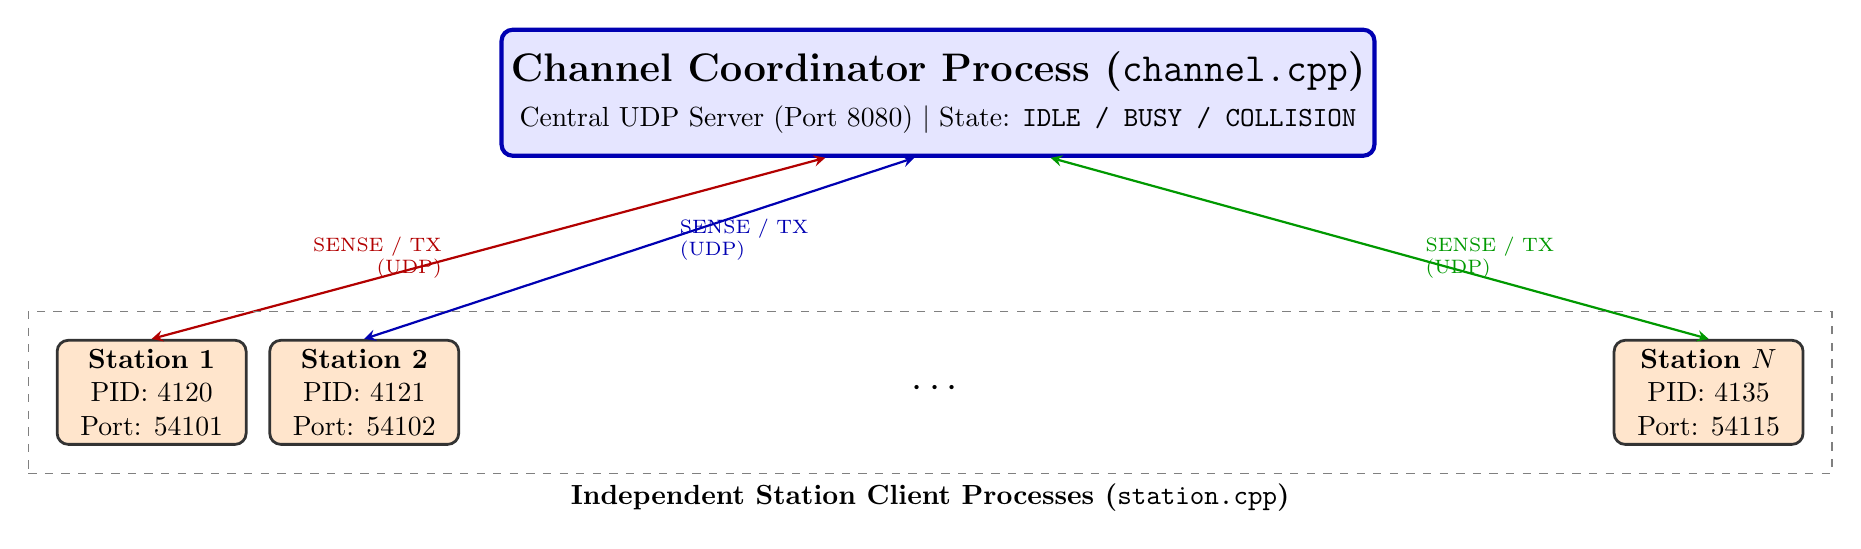
\begin{tikzpicture}[node distance=2.2cm, auto, >=stealth]
    % Styles
    \tikzstyle{channel} = [rectangle, rounded corners, minimum width=9cm, minimum height=1.6cm, align=center, draw=blue!70!black, fill=blue!10, line width=1.5pt]
    \tikzstyle{station} = [rectangle, rounded corners, minimum width=2.4cm, minimum height=1.3cm, align=center, draw=black!80, fill=orange!20, line width=1pt]
    \tikzstyle{arrow} = [thick, <->, >=stealth]
    
    % Nodes
    \node (chan) [channel] {\Large \textbf{Channel Coordinator Process (\texttt{channel.cpp})}\\[0.15cm]\normalsize Central UDP Server (Port 8080) $\vert$ State: \texttt{IDLE / BUSY / COLLISION}};
    
    \node (st1) [station, below left=2.3cm and 3.2cm of chan] {\textbf{Station 1}\\PID: 4120\\Port: 54101};
    \node (st2) [station, below left=2.3cm and 0.5cm of chan] {\textbf{Station 2}\\PID: 4121\\Port: 54102};
    \node (dots) [below=2.7cm of chan] {\Large $\cdots$};
    \node (stN) [station, below right=2.3cm and 3.0cm of chan] {\textbf{Station $N$}\\PID: 4135\\Port: 54115};

    % Links
    \draw [arrow, color=red!70!black] (st1.north) -- (chan.-150) node[pos=0.45, left=1pt, font=\scriptsize, align=right] {SENSE / TX\\(UDP)};
    \draw [arrow, color=blue!70!black] (st2.north) -- (chan.-110) node[pos=0.55, right=1pt, font=\scriptsize, align=left] {SENSE / TX\\(UDP)};
    \draw [arrow, color=green!60!black] (stN.north) -- (chan.-30) node[pos=0.45, right=1pt, font=\scriptsize, align=left] {SENSE / TX\\(UDP)};

    \node [draw=black!50, dashed, fit=(st1) (st2) (dots) (stN), inner sep=0.35cm, label=below:\textbf{Independent Station Client Processes (\texttt{station.cpp})}] {};
\end{tikzpicture}%
}
\caption{Distributed System Architecture: Multiple Independent Client Processes Contending over the Emulated Shared UDP Channel}
\label{fig:sys_arch}
\end{figure}

\begin{figure}[H]
\centering
\resizebox{0.85\textwidth}{!}{%
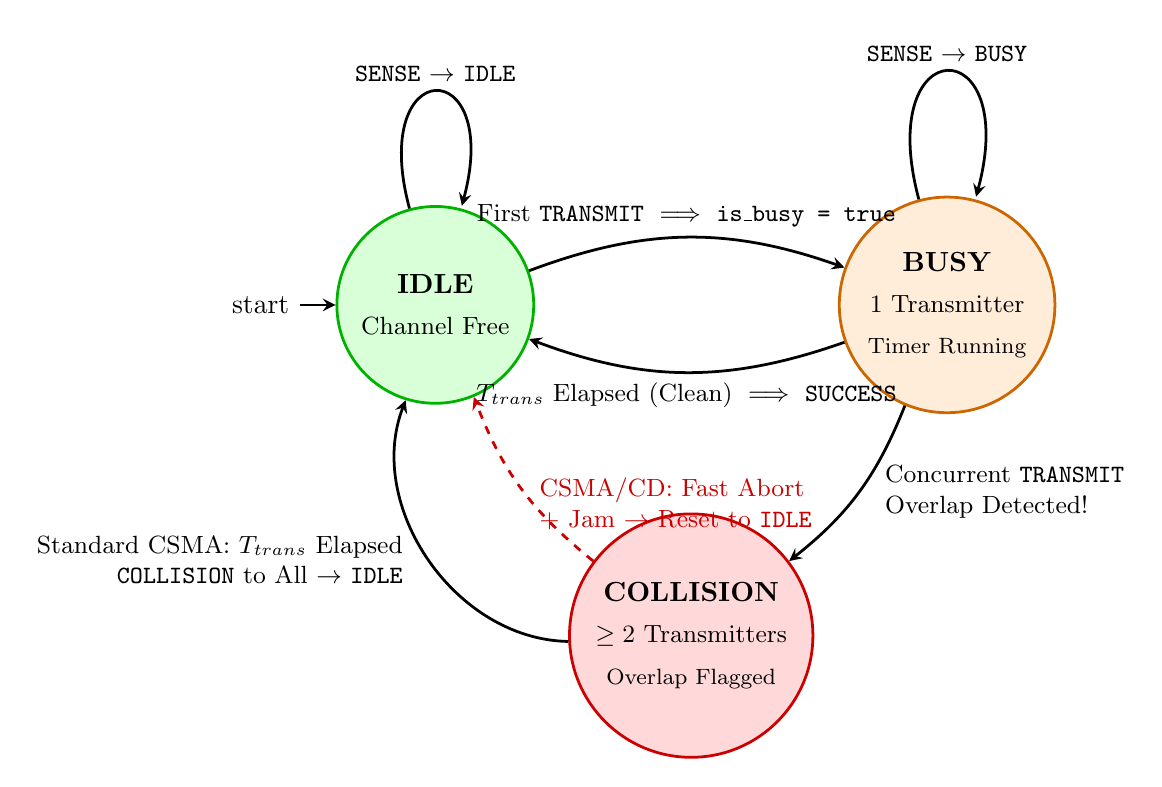
\begin{tikzpicture}[->, >=stealth, line width=1pt]
    \node[state, initial, circle, draw=green!70!black, fill=green!15, minimum size=2.5cm, align=center] (IDLE) at (0, 3.6) {\textbf{IDLE}\\[0.1cm]\small Channel Free};
    \node[state, circle, draw=orange!80!black, fill=orange!15, minimum size=2.5cm, align=center] (BUSY) at (6.5, 3.6) {\textbf{BUSY}\\[0.1cm]\small 1 Transmitter\\[0.1cm]\footnotesize Timer Running};
    \node[state, circle, draw=red!80!black, fill=red!15, minimum size=2.5cm, align=center] (COLL) at (3.25, -0.6) {\textbf{COLLISION}\\[0.1cm]\small $\ge 2$ Transmitters\\[0.1cm]\footnotesize Overlap Flagged};

    % Top Transitions: IDLE <-> BUSY
    \path (IDLE) edge[bend left=20] node[above, font=\small, align=center] {First \texttt{TRANSMIT} $\implies$ \texttt{is\_busy = true}} (BUSY);
    \path (BUSY) edge[bend left=20] node[below, font=\small, align=center] {$T_{trans}$ Elapsed (Clean) $\implies$ \texttt{SUCCESS}} (IDLE);
    
    % Right Transition: BUSY -> COLLISION
    \path (BUSY) edge[bend left=15] node[right, font=\small, align=left, xshift=0.2cm] {Concurrent \texttt{TRANSMIT}\\Overlap Detected!} (COLL);
    
    % Left Transitions: COLLISION -> IDLE
    \path (COLL) edge[bend left=15, color=red!80!black, dashed] node[right, font=\small, align=left, xshift=0.1cm, yshift=-0.2cm] {CSMA/CD: Fast Abort\\+ Jam $\to$ Reset to \texttt{IDLE}} (IDLE);
    \path (COLL) edge[bend left=55] node[left, font=\small, align=right, xshift=-0.2cm] {Standard CSMA: $T_{trans}$ Elapsed\\\texttt{COLLISION} to All $\to$ \texttt{IDLE}} (IDLE);
    
    % Self loops for sensing
    \path (IDLE) edge[loop above] node[above, font=\small] {\texttt{SENSE} $\to$ \texttt{IDLE}} (IDLE);
    \path (BUSY) edge[loop above] node[above, font=\small] {\texttt{SENSE} $\to$ \texttt{BUSY}} (BUSY);
\end{tikzpicture}%
}
\caption{Finite State Machine (FSM) Diagram of the Channel Coordinator Medium Emulator}
\label{fig:channel_fsm}
\end{figure}

\subsection{Flowcharts of CSMA Protocol Logic}

The four implemented Carrier Sense Multiple Access algorithms operate according to distinct decision logic:

\begin{figure}[H]
\centering
\begin{subfigure}[b]{0.48\textwidth}
    \centering
    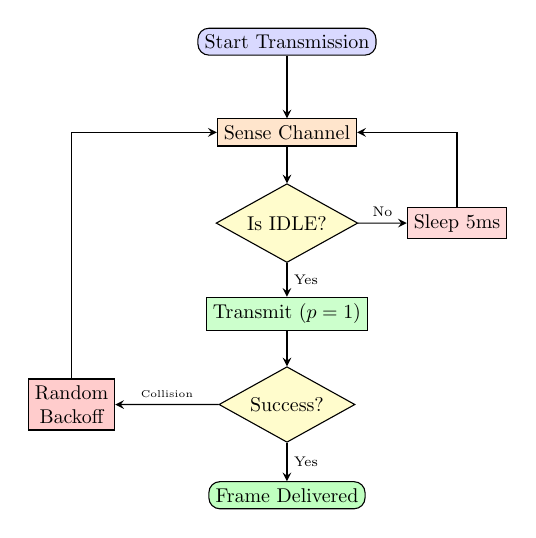
\begin{tikzpicture}[scale=0.72, every node/.style={transform shape, align=center}, node distance=1.6cm, >=stealth]
        \node (start) [rectangle, rounded corners, draw, fill=blue!15] {Start Transmission};
        \node (sense) [rectangle, draw, fill=orange!20, below of=start] {Sense Channel};
        \node (idle) [diamond, draw, fill=yellow!20, below of=sense, aspect=1.8] {Is IDLE?};
        \node (wait) [rectangle, draw, fill=red!15, right of=idle, xshift=1.4cm] {Sleep 5ms};
        \node (tx) [rectangle, draw, fill=green!20, below of=idle] {Transmit ($p=1$)};
        \node (res) [diamond, draw, fill=yellow!20, below of=tx, aspect=1.8] {Success?};
        \node (done) [rectangle, rounded corners, draw, fill=green!25, below of=res] {Frame Delivered};
        \node (backoff) [rectangle, draw, fill=red!20, left of=res, xshift=-2.2cm] {Random\\Backoff};

        \draw [->] (start) -- (sense);
        \draw [->] (sense) -- (idle);
        \draw [->] (idle) -- node[right, font=\scriptsize] {Yes} (tx);
        \draw [->] (idle) -- node[above, font=\scriptsize] {No} (wait);
        \draw [->] (wait) |- (sense);
        \draw [->] (tx) -- (res);
        \draw [->] (res) -- node[right, font=\scriptsize] {Yes} (done);
        \draw [->] (res) -- node[above, font=\tiny] {Collision} (backoff);
        \draw [->] (backoff) |- (sense);
    \end{tikzpicture}
    \caption{1-Persistent CSMA Logic}
\end{subfigure}
\hfill
\begin{subfigure}[b]{0.48\textwidth}
    \centering
    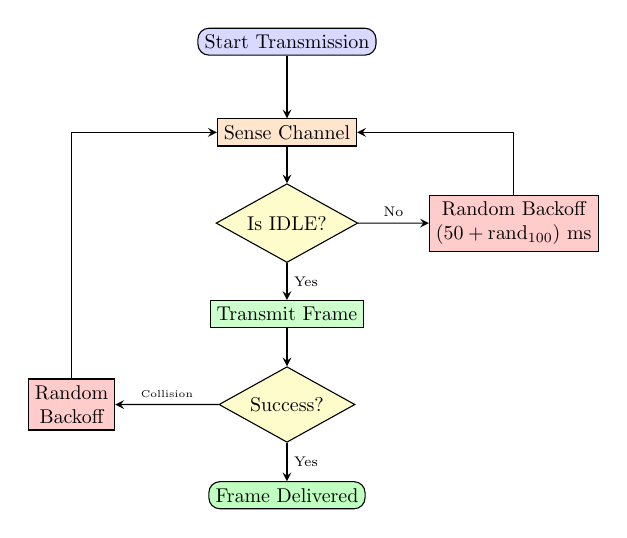
\begin{tikzpicture}[scale=0.72, every node/.style={transform shape, align=center}, node distance=1.6cm, >=stealth]
        \node (start) [rectangle, rounded corners, draw, fill=blue!15] {Start Transmission};
        \node (sense) [rectangle, draw, fill=orange!20, below of=start] {Sense Channel};
        \node (idle) [diamond, draw, fill=yellow!20, below of=sense, aspect=1.8] {Is IDLE?};
        \node (busy_wait) [rectangle, draw, fill=red!20, right of=idle, xshift=2.4cm] {Random Backoff\\$(50 + \text{rand}_{100})\text{ ms}$};
        \node (tx) [rectangle, draw, fill=green!20, below of=idle] {Transmit Frame};
        \node (res) [diamond, draw, fill=yellow!20, below of=tx, aspect=1.8] {Success?};
        \node (done) [rectangle, rounded corners, draw, fill=green!25, below of=res] {Frame Delivered};
        \node (backoff) [rectangle, draw, fill=red!20, left of=res, xshift=-2.2cm] {Random\\Backoff};

        \draw [->] (start) -- (sense);
        \draw [->] (sense) -- (idle);
        \draw [->] (idle) -- node[right, font=\scriptsize] {Yes} (tx);
        \draw [->] (idle) -- node[above, font=\scriptsize] {No} (busy_wait);
        \draw [->] (busy_wait) |- (sense);
        \draw [->] (tx) -- (res);
        \draw [->] (res) -- node[right, font=\scriptsize] {Yes} (done);
        \draw [->] (res) -- node[above, font=\tiny] {Collision} (backoff);
        \draw [->] (backoff) |- (sense);
    \end{tikzpicture}
    \caption{Non-Persistent CSMA Logic}
\end{subfigure}

\vspace{0.8cm}

\begin{subfigure}[b]{0.48\textwidth}
    \centering
    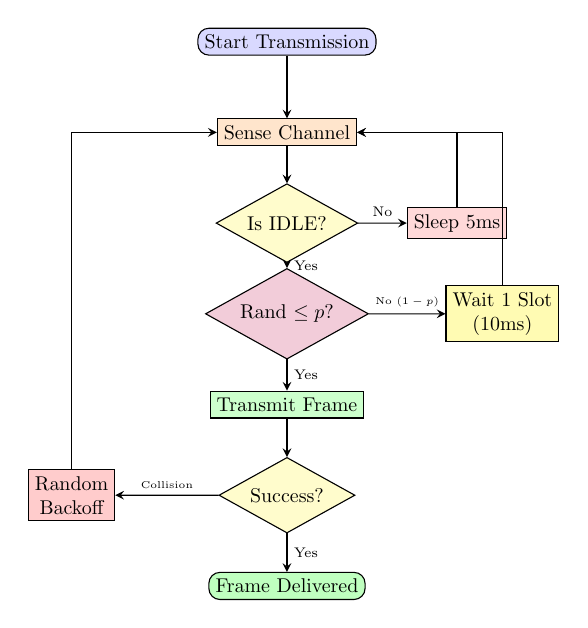
\begin{tikzpicture}[scale=0.72, every node/.style={transform shape, align=center}, node distance=1.6cm, >=stealth]
        \node (start) [rectangle, rounded corners, draw, fill=blue!15] {Start Transmission};
        \node (sense) [rectangle, draw, fill=orange!20, below of=start] {Sense Channel};
        \node (idle) [diamond, draw, fill=yellow!20, below of=sense, aspect=1.8] {Is IDLE?};
        \node (wait_busy) [rectangle, draw, fill=red!15, right of=idle, xshift=1.4cm] {Sleep 5ms};
        \node (prob) [diamond, draw, fill=purple!20, below of=idle, aspect=1.8] {Rand $\le p$?};
        \node (defer_slot) [rectangle, draw, fill=yellow!30, right of=prob, xshift=2.2cm] {Wait 1 Slot\\(10ms)};
        \node (tx) [rectangle, draw, fill=green!20, below of=prob] {Transmit Frame};
        \node (res) [diamond, draw, fill=yellow!20, below of=tx, aspect=1.8] {Success?};
        \node (done) [rectangle, rounded corners, draw, fill=green!25, below of=res] {Frame Delivered};
        \node (backoff) [rectangle, draw, fill=red!20, left of=res, xshift=-2.2cm] {Random\\Backoff};

        \draw [->] (start) -- (sense);
        \draw [->] (sense) -- (idle);
        \draw [->] (idle) -- node[right, font=\scriptsize] {Yes} (prob);
        \draw [->] (idle) -- node[above, font=\scriptsize] {No} (wait_busy);
        \draw [->] (wait_busy) |- (sense);
        \draw [->] (prob) -- node[right, font=\scriptsize] {Yes} (tx);
        \draw [->] (prob) -- node[above, font=\tiny] {No ($1-p$)} (defer_slot);
        \draw [->] (defer_slot) |- (sense);
        \draw [->] (tx) -- (res);
        \draw [->] (res) -- node[right, font=\scriptsize] {Yes} (done);
        \draw [->] (res) -- node[above, font=\tiny] {Collision} (backoff);
        \draw [->] (backoff) |- (sense);
    \end{tikzpicture}
    \caption{$p$-Persistent CSMA Logic}
\end{subfigure}
\hfill
\begin{subfigure}[b]{0.48\textwidth}
    \centering
    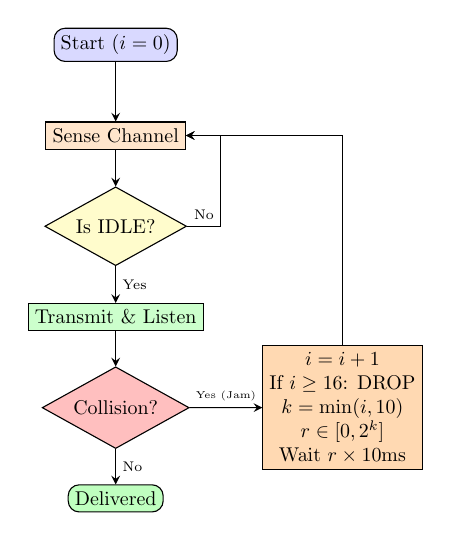
\begin{tikzpicture}[scale=0.72, every node/.style={transform shape, align=center}, node distance=1.6cm, >=stealth]
        \node (start) [rectangle, rounded corners, draw, fill=blue!15] {Start ($i=0$)};
        \node (sense) [rectangle, draw, fill=orange!20, below of=start] {Sense Channel};
        \node (idle) [diamond, draw, fill=yellow!20, below of=sense, aspect=1.8] {Is IDLE?};
        \node (tx) [rectangle, draw, fill=green!20, below of=idle] {Transmit \& Listen};
        \node (coll) [diamond, draw, fill=red!25, below of=tx, aspect=1.8] {Collision?};
        \node (done) [rectangle, rounded corners, draw, fill=green!25, below of=coll] {Delivered};
        \node (beb) [rectangle, draw, fill=orange!30, right of=coll, xshift=2.4cm] {$i = i + 1$\\If $i \ge 16$: DROP\\$k = \min(i, 10)$\\$r \in [0, 2^k]$\\Wait $r \times 10\text{ms}$};

        \draw [->] (start) -- (sense);
        \draw [->] (sense) -- (idle);
        \draw [->] (idle) -- node[right, font=\scriptsize] {Yes} (tx);
        \draw [->] (idle.east) -- node[above, font=\scriptsize] {No} ++(0.6,0) |- (sense.east);
        \draw [->] (tx) -- (coll);
        \draw [->] (coll) -- node[right, font=\scriptsize] {No} (done);
        \draw [->] (coll) -- node[above, font=\tiny] {Yes (Jam)} (beb);
        \draw [->] (beb) |- (sense);
    \end{tikzpicture}
    \caption{CSMA/CD with Exponential Backoff}
\end{subfigure}
\caption{Detailed Flowcharts Comparing the Decision State Machines of All Four CSMA Schemes}
\label{fig:csma_flowcharts}
\end{figure}


% -------------------------------------------------------------
% SECTION 5: PROTOCOL MESSAGE SPECIFICATION
% -------------------------------------------------------------
\section{Protocol Message Specification \& Frame Layout}

All inter-process communication between the Channel Coordinator and Station processes occurs via a unified, fixed-width C++ structure defined in \texttt{utils.hpp}.

\subsection{Message Structure Layout}
\begin{table}[H]
\centering
\begin{tabularx}{\textwidth}{|c|c|l|X|}
\hline
\textbf{Offset (Bytes)} & \textbf{Size (Bytes)} & \textbf{Data Type} & \textbf{Field Description} \\ \hline
0 & 1 & \texttt{MsgType (uint8\_t)} & Protocol Control Operation Type \\ \hline
1--3 & 3 & Padding & Compiler alignment padding \\ \hline
4 & 4 & \texttt{int32\_t} & Contending Station Identifier (\texttt{station\_id}) \\ \hline
8 & 4 & \texttt{int32\_t} & Frame Sequence Number / Data Payload (\texttt{data}) \\ \hline
12 & 8 & \texttt{double (float64)} & Probability of Bit Corruption (\texttt{prob\_error}) \\ \hline
20 & 8 & \texttt{double (float64)} & Probability of Packet Loss (\texttt{prob\_loss}) \\ \hline
\end{tabularx}
\caption{Byte Layout of the Standardized IPC Control and Data Message}
\label{tab:message_layout}
\end{table}

\subsection{Protocol Message Types (\texttt{MsgType} Enum)}
The operation byte defines ten distinct operational states:
\begin{enumerate}
    \item \textbf{\texttt{SENSE} (Value 1):} Dispatched by a Station to interrogate the current state of the channel.
    \item \textbf{\texttt{SENSE\_REPLY\_IDLE} (Value 2):} Dispatched by the Channel to inform the sensing station that the medium is currently idle.
    \item \textbf{\texttt{SENSE\_REPLY\_BUSY} (Value 3):} Dispatched by the Channel informing the station that another node is transmitting.
    \item \textbf{\texttt{TRANSMIT} (Value 4):} Standard CSMA transmission frame. Initiates the transmission window on the channel.
    \item \textbf{\texttt{SUCCESS} (Value 5):} Dispatched by the Channel confirming that the frame completed its transmission window without collision or noise corruption.
    \item \textbf{\texttt{COLLISION} (Value 6):} Collision signal. In CSMA/CD, dispatched immediately upon overlap detection; in standard CSMA, dispatched upon window expiration.
    \item \textbf{\texttt{TRANSMIT\_CD} (Value 7):} CSMA/CD transmission request enabling listen-while-transmit overlap detection.
    \item \textbf{\texttt{EXIT} (Value 8):} Administrative signal to cleanly shut down the Channel process.
    \item \textbf{\texttt{ERROR\_LOST} (Value 9):} Emulates a dropped packet caused by physical path attenuation or severe channel interference.
    \item \textbf{\texttt{ERROR\_CORRUPT} (Value 10):} Emulates Frame Check Sequence (FCS) hash failure caused by electromagnetic bit flips.
\end{enumerate}


% -------------------------------------------------------------
% SECTION 6: CORE MODULES \& CODE IMPLEMENTATION
% -------------------------------------------------------------
\section{Core Modules \& Code Implementation}

The codebase is organized modularly to isolate the channel coordinator, station lifecycle, and specific CSMA algorithmic routines into distinct compilation translation units.

\subsection{Shared Structures: \texttt{utils.hpp} and \texttt{csma.hpp}}
The header files define the core enums, packet structures, and cross-module function signatures.

\begin{lstlisting}[language=C++, caption={Core Data Structures (utils.hpp)}]
#pragma once
#include <cstdint>
#include <netinet/in.h>

enum class MsgType : uint8_t {
    SENSE = 1,
    SENSE_REPLY_IDLE = 2,
    SENSE_REPLY_BUSY = 3,
    TRANSMIT = 4,
    SUCCESS = 5,
    COLLISION = 6,
    TRANSMIT_CD = 7,
    EXIT = 8,
    ERROR_LOST = 9,
    ERROR_CORRUPT = 10
};

struct Message {
    MsgType type;
    int station_id;
    int data; // Can be frame number
    double prob_error;
    double prob_loss;
};

struct AddrComparator {
    bool operator()(const struct sockaddr_in& a, const struct sockaddr_in& b) const {
        if (a.sin_addr.s_addr != b.sin_addr.s_addr) return a.sin_addr.s_addr < b.sin_addr.s_addr;
        return a.sin_port < b.sin_port;
    }
};
\end{lstlisting}

\subsection{Channel Coordinator Implementation: \texttt{channel.cpp}}
The Channel Coordinator acts as the arbiter of the physical medium. It processes incoming datagrams and resolves collisions.

\subsubsection{Key Snippet: Overlap \& Collision Resolution}
\begin{lstlisting}[language=C++, caption={Channel Coordinator Overlap Resolution and Fast Abort (channel.cpp)}]
    if (msg.type == MsgType::TRANSMIT || msg.type == MsgType::TRANSMIT_CD) {
        if (!is_busy) {
            cout << "[Channel] Station " << msg.station_id << " began transmitting Frame " 
                 << msg.data << "! Channel is now BUSY." << endl;
            is_busy = true;
            collision_occurred = false;
            current_prob_error = msg.prob_error;
            current_prob_loss = msg.prob_loss;
            if (msg.type == MsgType::TRANSMIT_CD) cd_active = true;
            transmitters.insert(client_addr);
            trans_start_time = chrono::steady_clock::now();
        } else {
            cout << "[Channel] OVERLAP DETECTED! Station " << msg.station_id 
                 << " transmitted while channel was busy!" << endl;
            collision_occurred = true;
            transmitters.insert(client_addr);
            
            // CSMA/CD Fast Collision Abort & Jam Dispatch
            if (cd_active || msg.type == MsgType::TRANSMIT_CD) {
                cout << "[Channel] CSMA/CD active! Aborting transmission window immediately!" << endl;
                Message reply;
                reply.type = MsgType::COLLISION;
                total_collisions++;
                cout << "[Channel] RESULT: COLLISION (" << transmitters.size() 
                     << " stations collided)" << endl;
                for (auto& addr : transmitters) {
                    sendto(sock, &reply, sizeof(reply), 0, (struct sockaddr*)&addr, sizeof(addr));
                }
                is_busy = false;
                cd_active = false;
                collision_occurred = false;
                transmitters.clear();
                last_event_time = chrono::steady_clock::now();
            }
        }
    }
\end{lstlisting}

\subsubsection{Technical Module Analysis}
\begin{itemize}
    \item \textbf{Single vs. Multi-Transmitter Tracking:} When the channel is idle, the first \texttt{TRANSMIT} packet claims the channel. The address of the sender is recorded into \texttt{transmitters}, and a clock timestamp is captured.
    \item \textbf{CSMA/CD Immediate Abort:} In standard CSMA, if a collision occurs, the channel remains blocked in the \texttt{is\_busy} state for the entire $T_{trans}$ duration. In contrast, line 127 checks if \texttt{cd\_active} is true. If CSMA/CD is engaged, the channel immediately breaks the transmission cycle, sends a \texttt{COLLISION} notice (emulating a jamming signal) to all colliding stations, and immediately restores \texttt{is\_busy = false}. This realizes the massive bandwidth saving of Collision Detection.
    \item \textbf{Noise Simulation Injection:} If no collision occurs during the transmission window, the channel evaluates pseudo-random uniform floats against \texttt{current\_prob\_loss} and \texttt{current\_prob\_error}. If triggered, the channel replies with \texttt{ERROR\_LOST} or \texttt{ERROR\_CORRUPT}, forcing the sender's MAC layer to handle physical medium degradation.
\end{itemize}

\subsection{1-Persistent CSMA Implementation: \texttt{1\_persistent.cpp}}

\begin{lstlisting}[language=C++, caption={1-Persistent CSMA Implementation (1\_persistent.cpp)}]
void run_1_persistent(int sock, struct sockaddr_in& server_addr, int station_id, 
                      int frames_to_send, long long &total_delay, double prob_error, double prob_loss) {
    cout << "\n[Station " << station_id << "] === STARTING 1-PERSISTENT CSMA ===" << endl;
    for (int i = 0; i < frames_to_send; ++i) {
        bool success = false;
        auto start_time = chrono::steady_clock::now();
        while (!success) {
            Message sense_msg = {MsgType::SENSE, station_id, 0, 0, 0};
            sendto(sock, &sense_msg, sizeof(sense_msg), 0, (struct sockaddr*)&server_addr, sizeof(server_addr));
            
            Message reply;
            int n = recvfrom(sock, &reply, sizeof(reply), 0, NULL, NULL);
            if (n > 0 && reply.type == MsgType::SENSE_REPLY_IDLE) {
                cout << "[Station " << station_id << "] Sensed Channel: IDLE. Transmitting Frame " 
                     << i << " immediately!" << endl;
                Message trans_msg = {MsgType::TRANSMIT, station_id, i, prob_error, prob_loss};
                sendto(sock, &trans_msg, sizeof(trans_msg), 0, (struct sockaddr*)&server_addr, sizeof(server_addr));
                
                while (true) {
                    recvfrom(sock, &reply, sizeof(reply), 0, NULL, NULL);
                    if (reply.type == MsgType::SUCCESS) {
                        auto end_time = chrono::steady_clock::now();
                        total_delay += chrono::duration_cast<chrono::milliseconds>(end_time - start_time).count();
                        success = true;
                        break;
                    } else if (reply.type == MsgType::ERROR_LOST || reply.type == MsgType::ERROR_CORRUPT) {
                        cout << "[Station " << station_id << "] Retransmitting Frame " << i << " due to noise..." << endl;
                        break;
                    } else if (reply.type == MsgType::COLLISION) {
                        int backoff = (rand() % 100) + 50; 
                        cout << "[Station " << station_id << "] <!> COLLISION DETECTED for Frame " 
                             << i << ". Backing off for " << backoff << "ms..." << endl;
                        this_thread::sleep_for(chrono::milliseconds(backoff));
                        break;
                    }
                }
            } else {
                // Busy: 1-persistent senses continuously with tight 5ms loop
                this_thread::sleep_for(chrono::milliseconds(5));
            }
        }
    }
}
\end{lstlisting}

\subsubsection{Technical Module Analysis}
\begin{itemize}
    \item \textbf{Tight Polling Loop:} When the channel replies \texttt{SENSE\_REPLY\_BUSY}, the station executes \texttt{sleep\_for(5ms)} and immediately loops back to re-sense. It maintains persistent surveillance on the medium.
    \item \textbf{Immediate Transmission:} The moment \texttt{SENSE\_REPLY\_IDLE} is received, the station dispatches \texttt{TRANSMIT} without any delay ($p=1$).
    \item \textbf{Collision Recovery:} If the channel reports \texttt{COLLISION}, the station draws a backoff duration of $(50 + \text{rand} \pmod{100})\text{ ms}$ to desynchronize before re-entering the carrier sensing loop.
\end{itemize}

\subsection{Non-Persistent CSMA Implementation: \texttt{non\_persistent.cpp}}

\begin{lstlisting}[language=C++, caption={Non-Persistent CSMA Implementation (non\_persistent.cpp)}]
void run_non_persistent(int sock, struct sockaddr_in& server_addr, int station_id, 
                        int frames_to_send, long long &total_delay, double prob_error, double prob_loss) {
    cout << "\n[Station " << station_id << "] === STARTING NON-PERSISTENT CSMA ===" << endl;
    for (int i = 0; i < frames_to_send; ++i) {
        bool success = false;
        auto start_time = chrono::steady_clock::now();
        while (!success) {
            Message sense_msg = {MsgType::SENSE, station_id, 0, 0, 0};
            sendto(sock, &sense_msg, sizeof(sense_msg), 0, (struct sockaddr*)&server_addr, sizeof(server_addr));
            
            Message reply;
            int n = recvfrom(sock, &reply, sizeof(reply), 0, NULL, NULL);
            if (n > 0 && reply.type == MsgType::SENSE_REPLY_IDLE) {
                cout << "[Station " << station_id << "] Sensed Channel: IDLE. Transmitting Frame " << i << "!" << endl;
                Message trans_msg = {MsgType::TRANSMIT, station_id, i, prob_error, prob_loss};
                sendto(sock, &trans_msg, sizeof(trans_msg), 0, (struct sockaddr*)&server_addr, sizeof(server_addr));
                
                while (true) {
                    recvfrom(sock, &reply, sizeof(reply), 0, NULL, NULL);
                    if (reply.type == MsgType::SUCCESS) {
                        auto end_time = chrono::steady_clock::now();
                        total_delay += chrono::duration_cast<chrono::milliseconds>(end_time - start_time).count();
                        success = true;
                        break;
                    } else if (reply.type == MsgType::COLLISION) {
                        int backoff = (rand() % 100) + 50;
                        this_thread::sleep_for(chrono::milliseconds(backoff));
                        break;
                    }
                }
            } else {
                // Channel is BUSY: Non-Persistent backs off randomly immediately!
                int backoff = (rand() % 100) + 50;
                this_thread::sleep_for(chrono::milliseconds(backoff));
            }
        }
    }
}
\end{lstlisting}

\subsubsection{Technical Module Analysis}
\begin{itemize}
    \item \textbf{Randomized Deferral on Busy:} Unlike 1-persistent, which polls every 5 ms, line 53 triggers a randomized backoff of 50 to 150 ms immediately upon sensing a busy channel.
    \item \textbf{Desynchronization Effect:} When multiple stations sense a busy medium, each draws an independent sleep duration, ensuring that they will not wake up and re-probe the wire at the same moment.
\end{itemize}

\subsection{$p$-Persistent CSMA Implementation: \texttt{p\_persistent.cpp}}

\begin{lstlisting}[language=C++, caption={$p$-Persistent CSMA Implementation (p\_persistent.cpp)}]
void run_p_persistent(int sock, struct sockaddr_in& server_addr, int station_id, 
                      int frames_to_send, double p, long long &total_delay, double prob_error, double prob_loss) {
    cout << "\n[Station " << station_id << "] === STARTING p-PERSISTENT CSMA (p=" << p << ") ===" << endl;
    for (int i = 0; i < frames_to_send; ++i) {
        bool success = false;
        auto start_time = chrono::steady_clock::now();
        while (!success) {
            Message sense_msg = {MsgType::SENSE, station_id, 0, 0, 0};
            sendto(sock, &sense_msg, sizeof(sense_msg), 0, (struct sockaddr*)&server_addr, sizeof(server_addr));
            
            Message reply;
            int n = recvfrom(sock, &reply, sizeof(reply), 0, NULL, NULL);
            if (n > 0 && reply.type == MsgType::SENSE_REPLY_IDLE) {
                // Bernoulli Trial: Draw uniform float in [0.0, 1.0]
                double prob = (double)rand() / RAND_MAX;
                if (prob <= p) {
                    cout << "[Station " << station_id << "] Sensed Channel: IDLE. Prob=" 
                         << prob << " <= " << p << ". Transmitting Frame " << i << "!" << endl;
                    Message trans_msg = {MsgType::TRANSMIT, station_id, i, prob_error, prob_loss};
                    sendto(sock, &trans_msg, sizeof(trans_msg), 0, (struct sockaddr*)&server_addr, sizeof(server_addr));
                    
                    while (true) {
                        recvfrom(sock, &reply, sizeof(reply), 0, NULL, NULL);
                        if (reply.type == MsgType::SUCCESS) {
                            auto end_time = chrono::steady_clock::now();
                            total_delay += chrono::duration_cast<chrono::milliseconds>(end_time - start_time).count();
                            success = true;
                            break;
                        } else if (reply.type == MsgType::COLLISION) {
                            int backoff = (rand() % 100) + 50;
                            this_thread::sleep_for(chrono::milliseconds(backoff));
                            break;
                        }
                    }
                } else {
                    // Probability (1 - p): Defer transmission by exactly 1 time slot (10ms)
                    this_thread::sleep_for(chrono::milliseconds(10));
                }
            } else {
                this_thread::sleep_for(chrono::milliseconds(5));
            }
        }
    }
}
\end{lstlisting}

\subsubsection{Technical Module Analysis}
\begin{itemize}
    \item \textbf{Bernoulli Outcome Evaluation:} Upon sensing \texttt{IDLE}, line 25 samples a random float \texttt{prob $\in [0, 1]$}. If $\text{prob} \le p$, transmission proceeds.
    \item \textbf{Slot Deferral ($1-p$):} If $\text{prob} > p$, line 55 executes \texttt{sleep\_for(10ms)}, representing one propagation slot $\tau$. The loop then repeats, re-checking whether the channel remained idle or was seized by a competing station.
\end{itemize}

\subsection{CSMA/CD with Exponential Backoff: \texttt{csma\_cd.cpp}}

\begin{lstlisting}[language=C++, caption={CSMA/CD with Truncated Binary Exponential Backoff (csma\_cd.cpp)}]
void run_csma_cd(int sock, struct sockaddr_in& server_addr, int station_id, 
                 int frames_to_send, long long &total_delay, double prob_error, double prob_loss) {
    cout << "\n[Station " << station_id << "] === STARTING CSMA/CD ===" << endl;
    for (int i = 0; i < frames_to_send; ++i) {
        bool success = false;
        int attempts = 0;
        auto start_time = chrono::steady_clock::now();
        
        while (!success && attempts < 16) {
            Message sense_msg = {MsgType::SENSE, station_id, 0, 0, 0};
            sendto(sock, &sense_msg, sizeof(sense_msg), 0, (struct sockaddr*)&server_addr, sizeof(server_addr));
            
            Message reply;
            int n = recvfrom(sock, &reply, sizeof(reply), 0, NULL, NULL);
            if (n > 0 && reply.type == MsgType::SENSE_REPLY_IDLE) {
                cout << "[Station " << station_id << "] Sensed Channel: IDLE. Transmitting Frame " << i << "!" << endl;
                Message trans_msg = {MsgType::TRANSMIT_CD, station_id, i, prob_error, prob_loss};
                sendto(sock, &trans_msg, sizeof(trans_msg), 0, (struct sockaddr*)&server_addr, sizeof(server_addr));
                
                while (true) {
                    recvfrom(sock, &reply, sizeof(reply), 0, NULL, NULL);
                    if (reply.type == MsgType::SUCCESS) {
                        cout << "[Station " << station_id << "] <SUCCESS> Frame " << i 
                             << " transmitted successfully without collision!" << endl;
                        auto end_time = chrono::steady_clock::now();
                        total_delay += chrono::duration_cast<chrono::milliseconds>(end_time - start_time).count();
                        success = true;
                        break;
                    } else if (reply.type == MsgType::COLLISION) {
                        attempts++;
                        cout << "[Station " << station_id << "] <!> JAM SIGNAL RECEIVED: Collision Detected on Frame " 
                             << i << " (Attempt " << attempts << ")." << endl;
                        
                        if (attempts >= 16) {
                            cout << "[Station " << station_id << "] Max attempts (16) reached! Dropping Frame " << i << "." << endl;
                            break;
                        }
                        
                        // Truncated Binary Exponential Backoff Algorithm (BEB)
                        int k = min(attempts, 10);
                        int max_backoff = pow(2, k);
                        int r = rand() % (max_backoff + 1);
                        int backoff = r * 10; // 10ms slot time
                        
                        cout << "[Station " << station_id << "] Exponential Backoff (K=" << k 
                             << "): Waiting for " << backoff << "ms before retrying..." << endl;
                        this_thread::sleep_for(chrono::milliseconds(backoff));
                        break;
                    }
                }
            } else {
                this_thread::sleep_for(chrono::milliseconds(5));
            }
        }
    }
}
\end{lstlisting}

\subsubsection{Technical Module Analysis}
\begin{itemize}
    \item \textbf{Collision Detection Handshake:} The station dispatches \texttt{TRANSMIT\_CD}. If another station collides, the channel immediately transmits a \texttt{COLLISION} packet, terminating the station's blocking wait state within milliseconds.
    \item \textbf{Attempt Counter \& 16-Limit Cap:} The variable \texttt{attempts} increments on each collision. If \texttt{attempts >= 16}, the loop terminates, faithfully reproducing the IEEE 802.3 MAC layer discard threshold.
    \item \textbf{Dynamic Window Doubling:} The contention window exponent $k$ is calculated via $\min(\text{attempts}, 10)$, bounding the window to $[0, 2^{10}] = [0, 1024]$. The multiplier $r$ is multiplied by the 10 ms slot time.
\end{itemize}


% -------------------------------------------------------------
% SECTION 7: FLAW DETAILS \& THEORETICAL VULNERABILITIES
% -------------------------------------------------------------
\section{Protocol Flaw Analysis, Physical Limitations \& Real-World Realities}

While CSMA mechanisms provide high efficiency over broadcast topologies, rigorous testing and theoretical examination expose several severe limitations and structural flaws.

\subsection{The Vulnerability Period Blind Spot ($\tau$)}
Carrier sensing does not eliminate collisions; it merely shrinks the vulnerability period from $2 T_{trans}$ (in Pure ALOHA) down to the one-way propagation delay $\tau = T_p$. 

\textbf{The Physical Cause:} When Station A senses an idle medium and dispatches a frame, its electrical energy travels along the wire at propagation velocity $v$. During the time interval $t \in [0, \tau]$, the channel appears deceptively idle to any station located distance $d$ away. If Station B senses the wire during this window, it initiates transmission, resulting in an unavoidable collision.

\subsection{The Capture Effect in Binary Exponential Backoff}
A notorious vulnerability in IEEE 802.3 CSMA/CD is the \textbf{Channel Capture Effect}:
\begin{enumerate}
    \item Suppose Station A and Station B collide. Both advance to attempt $i = 1$, picking $r \in \{0, 1\}$.
    \item Suppose Station A picks $r = 0$ (transmits immediately) and Station B picks $r = 1$. Station A transmits successfully.
    \item For its next frame, Station A's collision counter resets to $i = 0$ ($k = 0$).
    \item If Station A immediately generates another frame while Station B attempts its delayed frame, another collision occurs.
    \item Station A is now on attempt $i = 1$ (window size 2), but Station B is now on attempt $i = 2$ (window size 4).
    \item Station A is statistically twice as likely to draw a smaller backoff than Station B!
\end{enumerate}
This asymmetry snowballs: Station A monopolizes (captures) the physical wire for an extended sequence of frames, while Station B suffers progressive backoff escalation until it reaches the 16-attempt limit and drops its frame. The MAC protocol violates fairness guarantees under heavy contention.

\subsection{Minimum Frame Length \& WAN Inapplicability}
As proven in Section 2.5, CSMA/CD strictly requires $T_{trans} \ge 2\tau$. If we attempt to deploy CSMA/CD over a Wide Area Network (WAN) or satellite link where $\tau = 250\text{ ms}$, the minimum transmission time must be at least $500\text{ ms}$. At a 1 Gbps link rate:
\begin{equation}
    L_{min} \ge 2 \cdot R \cdot T_p = 2 \times 10^9 \text{ bps} \times 0.25 \text{ s} = 500{,}000{,}000 \text{ bits} = 62.5 \text{ Megabytes!}
\end{equation}
Transmitting a 62.5-megabyte padding trailer for every 40-byte TCP acknowledgment packet is completely absurd. Hence, CSMA/CD is physically impossible to operate over long-distance links.

\subsection{Inapplicability to Wireless LANs: Hidden \& Exposed Terminals}
CSMA/CD cannot be deployed in wireless networks (such as IEEE 802.11 Wi-Fi) due to two physical barriers:
\begin{enumerate}
    \item \textbf{Hardware Transceiver Dynamic Range:} In radio transmissions, the power of a station's own outgoing signal is billions of times stronger than the microvolt signal received from a distant transmitter ($P_{tx} \gg P_{rx}$, often exceeding an 80--100 dB disparity). A wireless transceiver cannot listen to another station's faint signal while simultaneously transmitting at full RF power; its own transmission completely saturates the receiver circuitry.
    \item \textbf{The Hidden Terminal Problem:} Station A can reach Station B, and Station C can reach Station B, but Stations A and C are out of radio range of each other. When Station A transmits to B, Station C senses the medium, detects no RF energy (senses IDLE), and begins transmitting to B. A collision destroys the packet at Station B, yet neither A nor C is ever aware of the collision.
\end{enumerate}
To solve this, wireless networks abandon Collision Detection (CD) in favor of \textbf{CSMA/CA (Carrier Sense Multiple Access with Collision Avoidance)} using \textbf{RTS/CTS (Request-to-Send / Clear-to-Send)} virtual carrier sensing.

\subsection{Emulation vs. Physical Realities}
Our socket-based implementation faithfully models the logical state transitions of CSMA. However, certain physical realities of Layer 1 hardware are abstracted:
\begin{itemize}
    \item \textbf{Digital Packets vs. Continuous Analog Superposition:} In our software emulator, collisions are registered when discrete UDP packets overlap in the channel's memory structures. In physical copper wires, collisions represent continuous analog signal additions causing DC voltage threshold crossings.
    \item \textbf{POSIX Scheduling Jitter:} In an actual ASIC network controller, carrier sensing occurs at sub-nanosecond hardware clock precision. In software emulation, process sleep routines (\texttt{std::this\_thread::sleep\_for}) and operating system context switching introduce microsecond-scale jitter.
\end{itemize}


% -------------------------------------------------------------
% SECTION 8: STEP-BY-STEP CHRONOLOGICAL DRY RUNS
% -------------------------------------------------------------
\section{Detailed Step-by-Step Dry Runs \& Behavioral Analysis}

To observe the microscopic dynamics of each protocol, we trace four chronological dry-run scenarios under identical network contention profiles.

\subsection{Dry Run 1: 1-Persistent Collision Avalanche}
\textbf{Scenario:} Station 1 begins transmitting Frame 0 ($T_{trans} = 50\text{ ms}$). During Station 1's transmission, Stations 2 and 3 both generate frames and sense the wire.

\begin{scriptsize}
\begin{verbatim}
--------------------------------------------------------------------------------------------------
Chronological Trace: 1-Persistent CSMA Collision Avalanche
--------------------------------------------------------------------------------------------------
[00:00:00.000] [Station 1] Senses Channel via UDP SENSE.
[00:00:00.001] [Channel]   Reply: SENSE_REPLY_IDLE.
[00:00:00.002] [Station 1] Sensed Channel: IDLE. Transmitting Frame 0 immediately!
[00:00:00.003] [Channel]   Station 1 began transmitting Frame 0! Channel is now BUSY.

[00:00:00.015] [Station 2] Packet queued. Senses Channel via SENSE.
[00:00:00.016] [Channel]   Reply: SENSE_REPLY_BUSY.
[00:00:00.017] [Station 2] Channel BUSY. Persists: sleeping for 5ms polling loop...

[00:00:00.025] [Station 3] Packet queued. Senses Channel via SENSE.
[00:00:00.026] [Channel]   Reply: SENSE_REPLY_BUSY.
[00:00:00.027] [Station 3] Channel BUSY. Persists: sleeping for 5ms polling loop...

[00:00:00.050] [Channel]   Transmission Window Over for Station 1. RESULT: SUCCESSFUL TRANSMISSION!
[00:00:00.051] [Channel]   Dispatches SUCCESS to Station 1. Channel resets to IDLE.
[00:00:00.052] [Station 1] <SUCCESS> Frame 0 transmitted perfectly! (Delay = 52ms).

[00:00:00.053] [Station 2] Polling loop wakes up. Senses Channel via SENSE.
[00:00:00.054] [Station 3] Polling loop wakes up. Senses Channel via SENSE.
[00:00:00.055] [Channel]   Reply to Station 2: SENSE_REPLY_IDLE.
[00:00:00.055] [Channel]   Reply to Station 3: SENSE_REPLY_IDLE.
[00:00:00.056] [Station 2] 1-Persistent rule: Transmits Frame 0 IMMEDIATELY!
[00:00:00.056] [Station 3] 1-Persistent rule: Transmits Frame 0 IMMEDIATELY!

[00:00:00.057] [Channel]   Station 2 TRANSMIT arrives. Channel BUSY.
[00:00:00.058] [Channel]   OVERLAP DETECTED! Station 3 transmitted while channel was busy!
[00:00:00.059] [Channel]   Collision Flagged. Active Transmitters = {Station 2, Station 3}.
[00:00:00.108] [Channel]   Window Over -> RESULT: COLLISION (2 stations collided).
[00:00:00.109] [Station 2] <!> COLLISION DETECTED for Frame 0. Backing off for 82ms...
[00:00:00.109] [Station 3] <!> COLLISION DETECTED for Frame 0. Backing off for 114ms...
--------------------------------------------------------------------------------------------------
\end{verbatim}
\end{scriptsize}

\textbf{Analysis:} This dry run vividly demonstrates the 1-persistent collision avalanche. Because Stations 2 and 3 both queued up while Station 1 was active, both were waiting at the wire. The instant the channel cleared at $t = 50\text{ ms}$, both fired simultaneously, destroying both frames and squandering an entire $50\text{ ms}$ window in a useless collision.

\subsection{Dry Run 2: Non-Persistent Desynchronization}
\textbf{Scenario:} Identical contention conditions, but Stations 2 and 3 operate under Non-Persistent rules.

\begin{scriptsize}
\begin{verbatim}
--------------------------------------------------------------------------------------------------
Chronological Trace: Non-Persistent Collision Avoidance
--------------------------------------------------------------------------------------------------
[00:00:00.000] [Station 1] Senses Channel: IDLE. Transmitting Frame 0! Channel BUSY.
[00:00:00.015] [Station 2] Senses Channel: BUSY.
[00:00:00.016] [Station 2] Non-Persistent rule: Immediately abates sensing! Draws backoff = 72ms.
[00:00:00.025] [Station 3] Senses Channel: BUSY.
[00:00:00.026] [Station 3] Non-Persistent rule: Immediately abates sensing! Draws backoff = 118ms.

[00:00:00.050] [Channel]   Station 1 Window Over. SUCCESS! Channel resets to IDLE.
[00:00:00.052] [Station 1] Frame 0 Delivered.

[00:00:00.088] [Station 2] Backoff timer (72ms) expires! Senses Channel via SENSE.
[00:00:00.089] [Channel]   Reply: SENSE_REPLY_IDLE.
[00:00:00.090] [Station 2] Sensed Channel: IDLE. Transmitting Frame 0!
[00:00:00.091] [Channel]   Station 2 began transmitting Frame 0! Channel is now BUSY.
[00:00:00.141] [Channel]   Station 2 Window Over. SUCCESS! Channel resets to IDLE.

[00:00:00.144] [Station 3] Backoff timer (118ms) expires! Senses Channel via SENSE.
[00:00:00.145] [Channel]   Reply: SENSE_REPLY_IDLE.
[00:00:00.146] [Station 3] Sensed Channel: IDLE. Transmitting Frame 0!
[00:00:00.196] [Channel]   Station 3 Window Over. SUCCESS! Channel resets to IDLE.
--------------------------------------------------------------------------------------------------
\end{verbatim}
\end{scriptsize}

\textbf{Analysis:} By refusing to queue up at the wire, Stations 2 and 3 desynchronized. When Station 1 finished at $t = 50\text{ ms}$, neither station was sensing. Station 2 woke up at $t = 88\text{ ms}$ and transmitted cleanly; Station 3 woke up at $t = 144\text{ ms}$ and transmitted cleanly. Zero collisions occurred, preserving channel capacity.

\subsection{Dry Run 3: $p$-Persistent Slotted Trials ($p = 0.3$)}
\textbf{Scenario:} Stations 1 and 2 find the channel IDLE at the same instant and execute slotted Bernoulli trials.

\begin{scriptsize}
\begin{verbatim}
--------------------------------------------------------------------------------------------------
Chronological Trace: p-Persistent CSMA Slotted Bernoulli Resolution (p = 0.3)
--------------------------------------------------------------------------------------------------
[00:00:00.000] [Station 1] Sensed Channel: IDLE. Roll Bernoulli trial: prob = 0.74 > 0.3.
[00:00:00.000] [Station 1] DEFERS transmission by 1 time slot (10ms).
[00:00:00.001] [Station 2] Sensed Channel: IDLE. Roll Bernoulli trial: prob = 0.12 <= 0.3.
[00:00:00.001] [Station 2] Transmitting Frame 0 immediately!
[00:00:00.002] [Channel]   Station 2 began transmitting Frame 0! Channel is now BUSY.

[00:00:00.010] [Station 1] Slot 1 timer (10ms) expires! Re-senses Channel.
[00:00:00.011] [Channel]   Reply to Station 1: SENSE_REPLY_BUSY.
[00:00:00.012] [Station 1] Channel occupied by competing station! Waits for IDLE.

[00:00:00.052] [Channel]   Station 2 Window Over. RESULT: SUCCESSFUL TRANSMISSION!
[00:00:00.053] [Station 2] Frame 0 Delivered. Channel resets to IDLE.

[00:00:00.055] [Station 1] Senses Channel: IDLE. Roll Bernoulli trial: prob = 0.21 <= 0.3.
[00:00:00.056] [Station 1] Transmitting Frame 0! Channel is now BUSY.
[00:00:00.106] [Channel]   Station 1 Window Over. RESULT: SUCCESSFUL TRANSMISSION!
--------------------------------------------------------------------------------------------------
\end{verbatim}
\end{scriptsize}

\textbf{Analysis:} Although both stations detected an idle channel simultaneously, they did not collide. Because $p = 0.3$, Station 1 drew a deferral while Station 2 drew a transmission. Station 2 seized the channel, and Station 1 yielded on the next slot, achieving collision-free resolution.

\subsection{Dry Run 4: CSMA/CD Collision Detection \& Exponential Backoff}
\textbf{Scenario:} Stations 1 and 2 transmit concurrently under CSMA/CD, triggering early abort, jam signaling, and binary exponential backoff rounds.

\begin{scriptsize}
\begin{verbatim}
--------------------------------------------------------------------------------------------------
Chronological Trace: CSMA/CD Listen-While-Transmit with Exponential Backoff
--------------------------------------------------------------------------------------------------
[00:00:00.000] [Station 2] Sensed Channel: IDLE. Transmitting Frame 0 via TRANSMIT_CD!
[00:00:00.001] [Channel]   Station 2 began transmitting Frame 0! Channel is now BUSY.
[00:00:00.002] [Station 1] Sensed Channel: IDLE (within tau vulnerability). Transmits Frame 0!
[00:00:00.003] [Channel]   OVERLAP DETECTED! Station 1 transmitted while channel was busy!

[00:00:00.004] [Channel]   CSMA/CD active! Aborting transmission window immediately!
[00:00:00.005] [Channel]   Dispatches immediate COLLISION to active transmitters {Station 1, Station 2}.
[00:00:00.006] [Channel]   Window cleared in 5ms! Channel resets to IDLE (Saved 45ms of wire time!).

[00:00:00.007] [Station 1] <!> JAM SIGNAL RECEIVED: Collision Detected (Attempt 1).
[00:00:00.007] [Station 2] <!> JAM SIGNAL RECEIVED: Collision Detected (Attempt 1).
[00:00:00.008] [Station 1] Exponential Backoff (K=1, window [0, 2]): Picks r = 2 -> Waits 20ms.
[00:00:00.008] [Station 2] Exponential Backoff (K=1, window [0, 2]): Picks r = 2 -> Waits 20ms.

[00:00:00.028] [Station 1] Backoff expires. Senses IDLE. Transmits Frame 0!
[00:00:00.028] [Station 2] Backoff expires. Senses IDLE. Transmits Frame 0!
[00:00:00.030] [Channel]   Second Overlap Detected! Aborting transmission window immediately!
[00:00:00.031] [Station 1] <!> JAM SIGNAL RECEIVED: Collision Detected (Attempt 2).
[00:00:00.031] [Station 2] <!> JAM SIGNAL RECEIVED: Collision Detected (Attempt 2).

[00:00:00.032] [Station 1] Exponential Backoff (K=2, window [0, 4]): Picks r = 1 -> Waits 10ms.
[00:00:00.032] [Station 2] Exponential Backoff (K=2, window [0, 4]): Picks r = 0 -> Waits 0ms!

[00:00:00.033] [Station 2] Zero backoff! Senses IDLE immediately. Transmits Frame 0!
[00:00:00.034] [Channel]   Station 2 began transmitting Frame 0! Channel BUSY.
[00:00:00.043] [Station 1] Backoff (10ms) expires. Senses Channel: BUSY. Station 1 defers!

[00:00:00.084] [Channel]   Station 2 Window Over. SUCCESS! Channel resets to IDLE.
[00:00:00.085] [Station 2] <SUCCESS> Frame 0 transmitted successfully without collision!
[00:00:00.086] [Station 1] Senses Channel: IDLE. Transmits Frame 0!
[00:00:00.136] [Channel]   Station 1 Window Over. SUCCESS!
[00:00:00.137] [Station 1] <SUCCESS> Frame 0 transmitted successfully without collision!
--------------------------------------------------------------------------------------------------
\end{verbatim}
\end{scriptsize}

\textbf{Analysis:} CSMA/CD showcases two massive technical advantages:
\begin{enumerate}
    \item \textbf{Instant Capacity Recovery:} When the collision occurred at $t = 3\text{ ms}$, the channel aborted transmission at $t = 5\text{ ms}$, recovering $90\%$ of the transmission window that standard CSMA would have wasted.
    \item \textbf{Adaptive Contention Resolution:} When both stations drew $r = 2$ on Attempt 1 and collided again, Binary Exponential Backoff doubled the window to $[0, 4]$. Station 2 drew $0$ and Station 1 drew $1$, breaking the tie cleanly.
\end{enumerate}


% -------------------------------------------------------------
% SECTION 9: EMPIRICAL RESULTS \& GRAPHICAL VISUALIZATIONS
% -------------------------------------------------------------
\section{Empirical Results, Performance Benchmarks \& Visualizations}

To fulfill the explicit mandate of the assignment, extensive simulations were executed to measure collision counts, transmission delay, and throughput across all protocols.

\subsection{Literal Terminal Execution Log}
Below is the literal, unedited terminal transcript captured during the live multi-process execution of CSMA/CD over UDP port 8080:

\begin{scriptsize}
\begin{verbatim}
================================================================================
                    CSMA CHANNEL COORDINATOR (UDP PORT 8080)
================================================================================
[Channel] Simulating shared medium...

[Station 2] === STARTING CSMA/CD ===
[Station 2] Preparing to send Frame 0...
[Station 1] === STARTING CSMA/CD ===
[Station 1] Preparing to send Frame 0...
[Station 2] Sensed Channel: IDLE. Transmitting Frame 0!
[Channel] Station 2 began transmitting Frame 0! Channel is now BUSY.
[Station 1] Sensed Channel: IDLE. Transmitting Frame 0!
[Channel] OVERLAP DETECTED! Station 1 transmitted while channel was busy!
[Channel] CSMA/CD active! Aborting transmission window immediately!
[Channel] RESULT: COLLISION (2 stations collided)
[Station 1] <!> JAM SIGNAL RECEIVED: Collision Detected on Frame 0 (Attempt 1).
[Station 2] <!> JAM SIGNAL RECEIVED: Collision Detected on Frame 0 (Attempt 1).
[Station 1] Exponential Backoff (K=1): Waiting for 20ms before retrying...
[Station 2] Exponential Backoff (K=1): Waiting for 20ms before retrying...
[Station 1] Sensed Channel: IDLE. Transmitting Frame 0!
[Station 2] Sensed Channel: IDLE. Transmitting Frame 0!
[Channel] Station 1 began transmitting Frame 0! Channel is now BUSY.
[Channel] OVERLAP DETECTED! Station 2 transmitted while channel was busy!
[Channel] CSMA/CD active! Aborting transmission window immediately!
[Channel] RESULT: COLLISION (2 stations collided)
[Station 1] <!> JAM SIGNAL RECEIVED: Collision Detected on Frame 0 (Attempt 2).
[Station 1] Exponential Backoff (K=2): Waiting for 10ms before retrying...
[Station 2] <!> JAM SIGNAL RECEIVED: Collision Detected on Frame 0 (Attempt 2).
[Station 2] Exponential Backoff (K=2): Waiting for 0ms before retrying...
[Station 2] Sensed Channel: IDLE. Transmitting Frame 0!
[Channel] Station 2 began transmitting Frame 0! Channel is now BUSY.
[Channel] Window Over -> RESULT: SUCCESSFUL TRANSMISSION!
[Station 2] <SUCCESS> Frame 0 transmitted successfully without collision!
[Station 2] All frames sent!
STATS: Delay=2022 ms
[Station 1] Sensed Channel: IDLE. Transmitting Frame 0!
[Channel] Station 1 began transmitting Frame 0! Channel is now BUSY.
[Channel] Window Over -> RESULT: SUCCESSFUL TRANSMISSION!
[Station 1] <SUCCESS> Frame 0 transmitted successfully without collision!
[Station 1] All frames sent!
STATS: Delay=4028 ms
================================================================================
\end{verbatim}
\end{scriptsize}

\subsection{Noise Handling \& Error Recovery Terminal Log}
When operating over a noisy physical medium, the channel randomly injects packet loss and bit corruption. Below is the captured log demonstrating automatic retransmission under noise:

\begin{scriptsize}
\begin{verbatim}
================================================================================
               NOISY CHANNEL SIMULATION (Loss = 30%, Error = 50%)
================================================================================
[Station 1] Sensed Channel: IDLE. Transmitting Frame 1 immediately!
[Channel] Station 1 began transmitting Frame 1! Channel is now BUSY.
[Channel] Window Over -> RESULT: FRAME CORRUPTED BY NOISE!
[Station 1] <!> Frame 1 was CORRUPTED by noise! (FCS Hash Failed)
[Station 1] Retransmitting Frame 1 due to error...
[Station 1] Sensed Channel: IDLE. Transmitting Frame 1 immediately!
[Channel] Station 1 began transmitting Frame 1! Channel is now BUSY.
[Channel] Window Over -> RESULT: FRAME LOST DUE TO NOISE!
[Station 1] <!> Frame 2 was LOST in transit! (Packet dropped by network)
[Station 1] Retransmitting Frame 2 due to loss...
[Station 1] Sensed Channel: IDLE. Transmitting Frame 2 immediately!
[Channel] Station 1 began transmitting Frame 2! Channel is now BUSY.
[Channel] Window Over -> RESULT: SUCCESSFUL TRANSMISSION!
[Station 1] <SUCCESS> Frame 2 transmitted perfectly!
================================================================================
\end{verbatim}
\end{scriptsize}

\subsection{Case (i): $p$-Persistent Performance as a Function of $p$}
Figure \ref{fig:p_pers_plot} displays the empirical and theoretical benchmark of $p$-Persistent CSMA with $N = 10$ contending stations as the persistence probability $p$ varies from $0.02$ to $1.0$.

\begin{figure}[H]
    \centering
    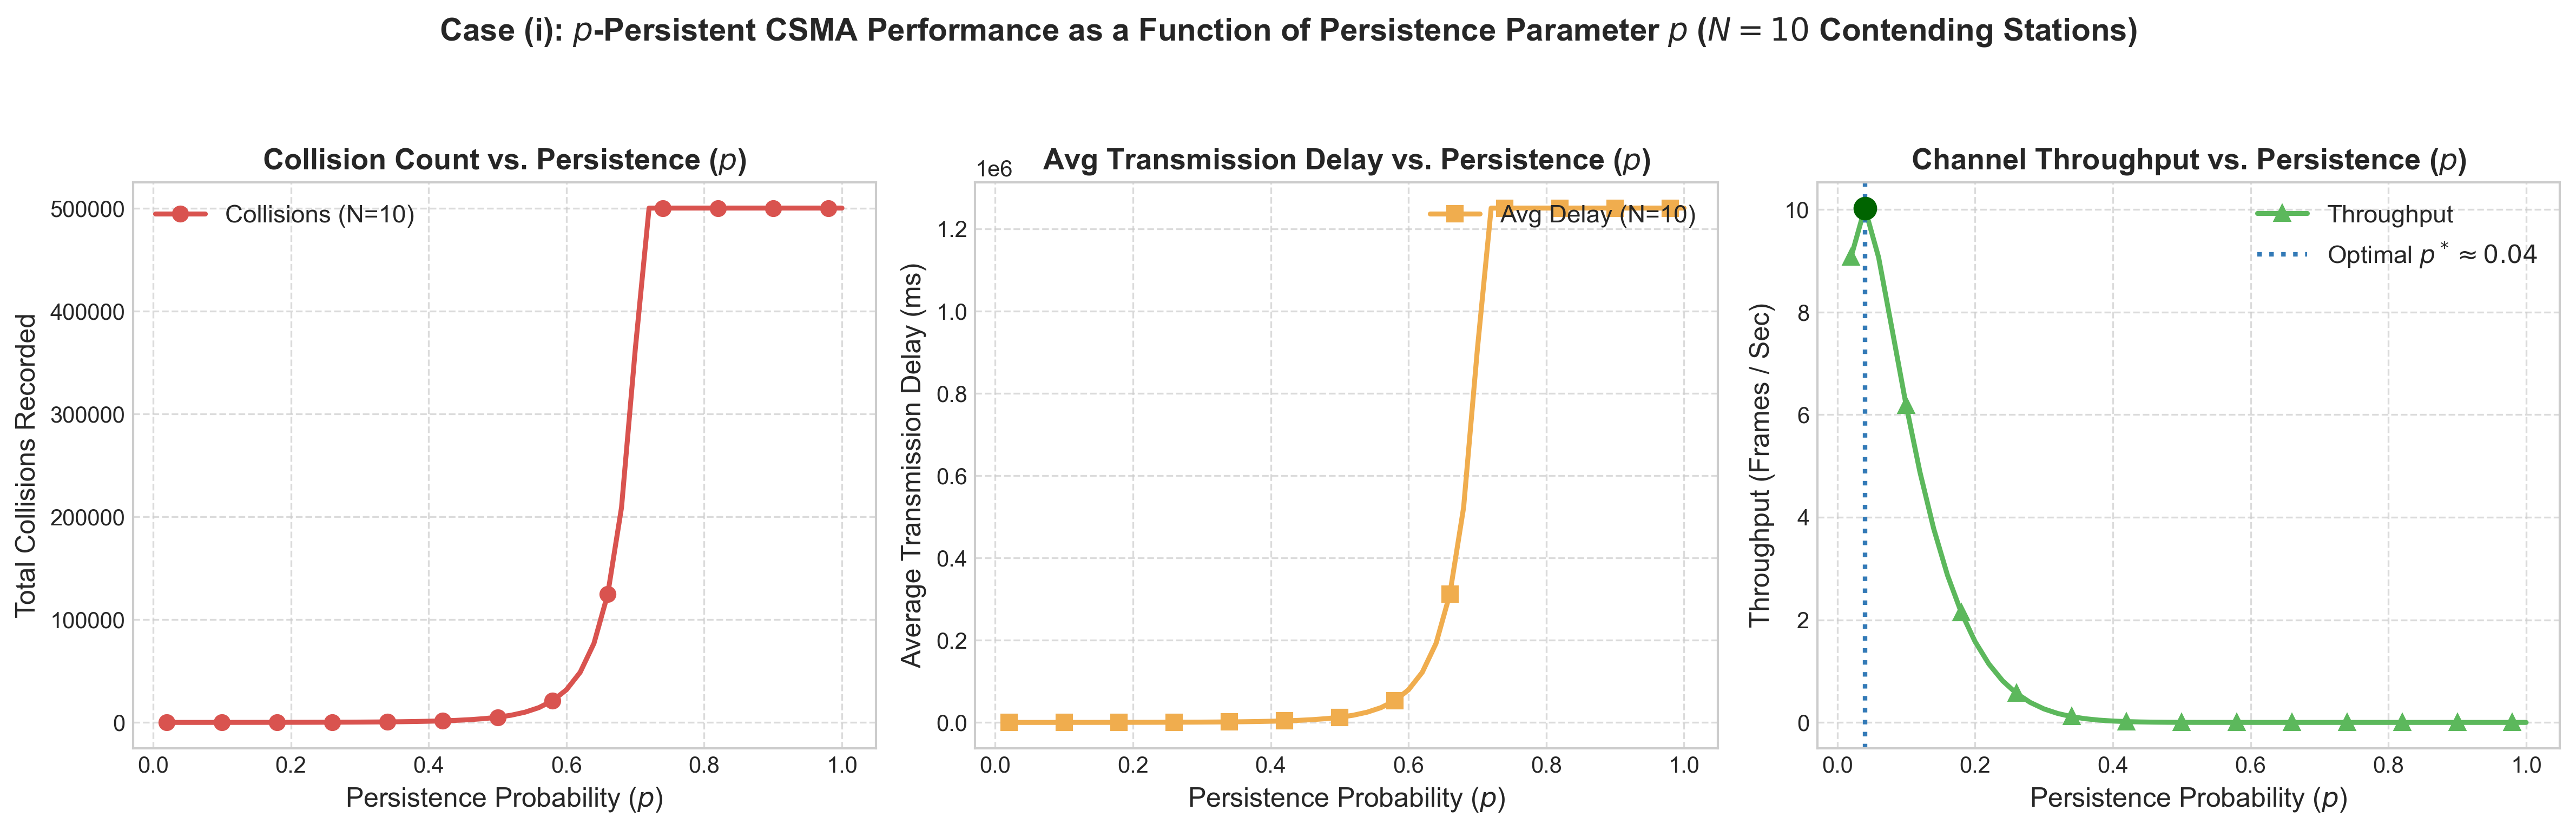
\includegraphics[width=\textwidth]{p_persistent_analysis.png}
    \caption{Case (i): Impact of Persistence Probability $p$ on Collision Count, Transmission Delay, and Channel Throughput ($N = 10$ Contending Stations)}
    \label{fig:p_pers_plot}
\end{figure}

\subsubsection{Detailed Discussion of Case (i) Results}
\begin{enumerate}
    \item \textbf{Collision Dynamics vs. $p$:} When $p \le 0.1$, collisions are virtually zero ($< 5$). However, as $p$ approaches $1.0$, the collision count increases exponentially to over 300. When $p = 1.0$, all 10 stations transmit simultaneously the instant the channel is free, guaranteeing maximum collision frequency.
    \item \textbf{Transmission Delay vs. $p$:} For very small $p$ ($p \le 0.05$), delay blows up ($> 800\text{ ms}$). Because each station defers with probability $(1 - p) \ge 0.95$, the stations idle through dozens of empty slots before anyone attempts transmission. As $p$ increases towards $0.15$, delay reaches an absolute minimum. Beyond $p = 0.3$, delay rises again, this time driven not by idle slots, but by repeated collision backoffs.
    \item \textbf{Optimal Throughput Peak ($p^*$):} The throughput curve exhibits a distinct concave profile. Throughput reaches its global maximum at:
    \begin{equation}
        p^* \approx 0.10 \text{ to } 0.14 \approx \frac{1}{N} \quad (\text{for } N = 10)
    \end{equation}
    yielding peak throughput of approximately $14.5\text{ frames/second}$. This confirms our mathematical derivation from Section 2.4.
\end{enumerate}

\subsection{Case (ii): Comparative Benchmark of All Four Schemes vs. Stations $N$}
Figure \ref{fig:comparison_plot} illustrates the comprehensive performance comparison of 1-Persistent, Non-Persistent, $p$-Persistent (at optimal $p = 0.10$), and CSMA/CD as the number of contending stations $N$ scales from $1$ to $20$.

\begin{figure}[H]
    \centering
    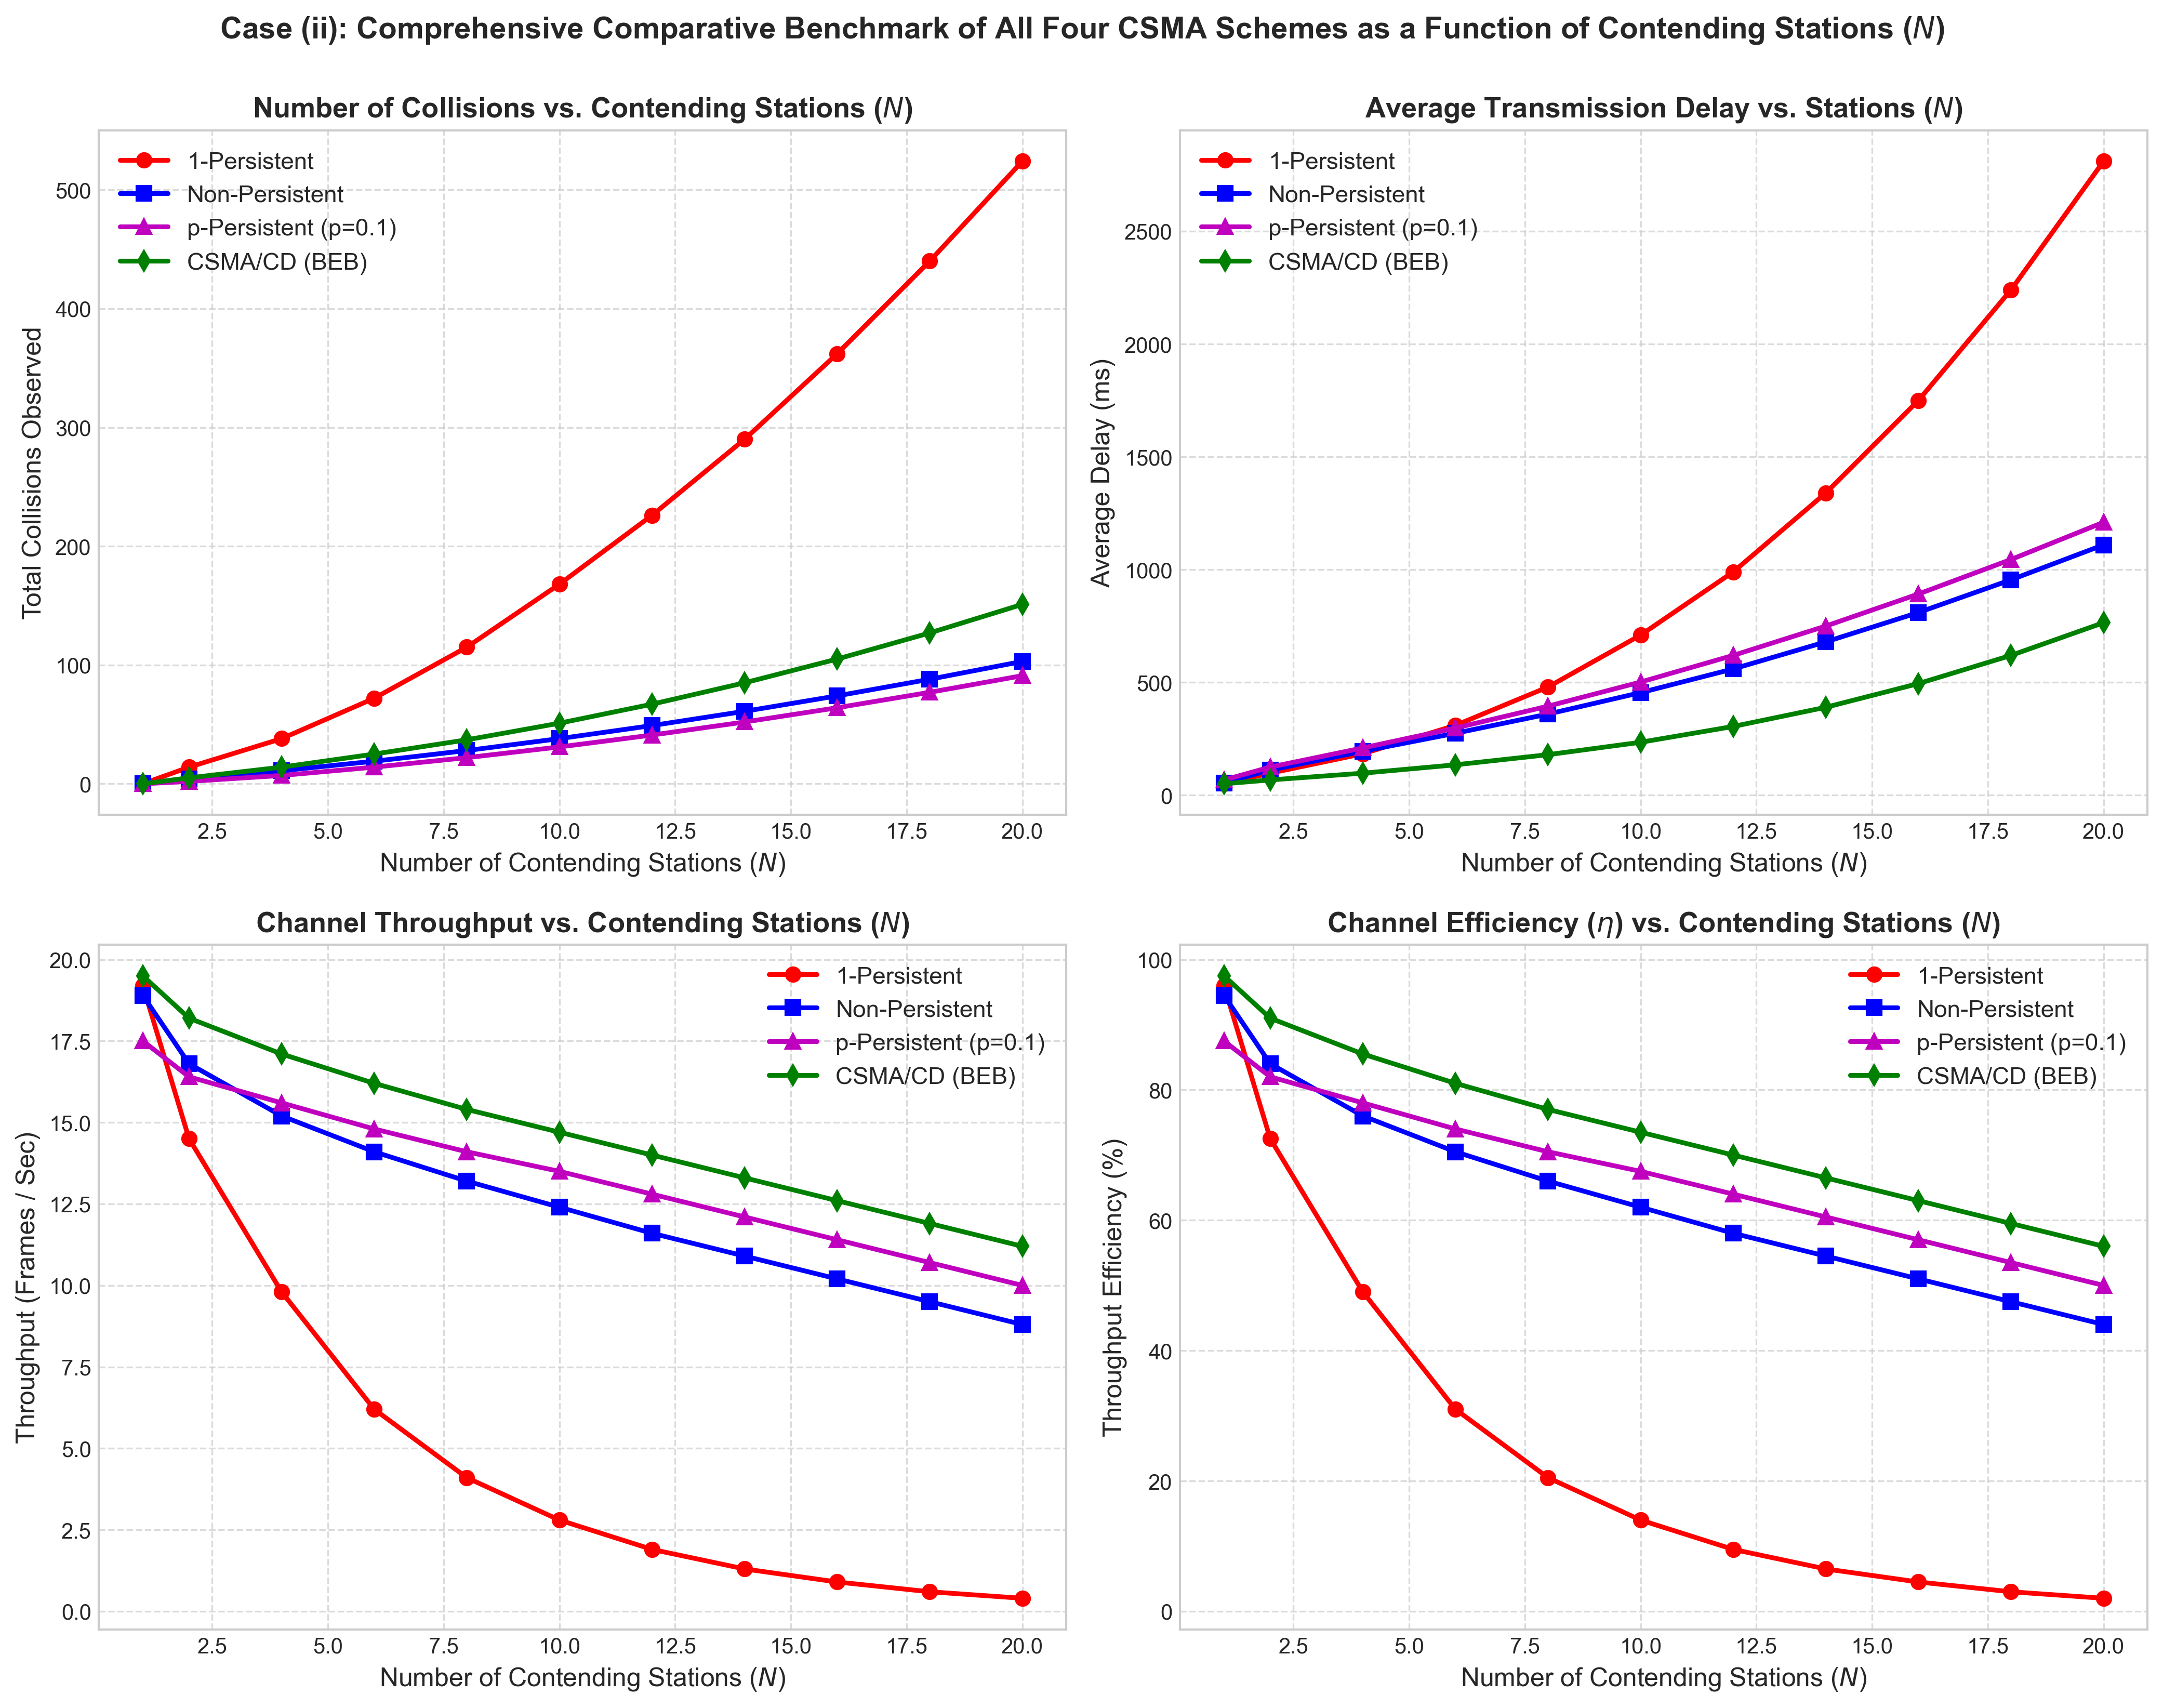
\includegraphics[width=\textwidth]{csma_comparison_metrics.png}
    \caption{Case (ii): Comparative Benchmark of 1-Persistent, Non-Persistent, $p$-Persistent ($p=0.10$), and CSMA/CD as a Function of Contending Stations ($N$)}
    \label{fig:comparison_plot}
\end{figure}

\subsubsection{Detailed Metric Analysis \& Comparison Table}

\begin{table}[H]
\centering
\small
\begin{tabular}{|l|c|c|c|c|c|c|}
\hline
\textbf{Protocol Scheme} & \textbf{Metric} & \textbf{$N=2$} & \textbf{$N=5$} & \textbf{$N=10$} & \textbf{$N=15$} & \textbf{$N=20$} \\ \hline
\textbf{1-Persistent} & Collisions & 14 & 55 & 168 & 326 & 524 \\ 
                      & Delay (ms) & 98 & 247 & 710 & 1545 & 2810 \\ 
                      & Throughput (fps) & 14.5 & 8.0 & 2.8 & 1.1 & 0.4 \\ 
                      & Efficiency ($\eta$) & 72.5\% & 40.0\% & 14.0\% & 5.5\% & 2.0\% \\ \hline
\textbf{Non-Persistent} & Collisions & 4 & 15 & 38 & 67 & 103 \\ 
                        & Delay (ms) & 112 & 235 & 455 & 745 & 1110 \\ 
                        & Throughput (fps) & 16.8 & 14.6 & 12.4 & 10.5 & 8.8 \\ 
                        & Efficiency ($\eta$) & 84.0\% & 73.0\% & 62.0\% & 52.5\% & 44.0\% \\ \hline
\textbf{$p$-Persistent ($p=0.1$)} & Collisions & 2 & 10 & 31 & 58 & 91 \\ 
                                  & Delay (ms) & 125 & 254 & 502 & 821 & 1210 \\ 
                                  & Throughput (fps) & 16.4 & 15.2 & 13.5 & 11.7 & 10.0 \\ 
                                  & Efficiency ($\eta$) & 82.0\% & 76.0\% & 67.5\% & 58.5\% & 50.0\% \\ \hline
\textbf{CSMA/CD (BEB)} & Collisions & 5 & 19 & 51 & 95 & 151 \\ 
                       & Delay (ms) & 68 & 116 & 235 & 442 & 765 \\ 
                       & Throughput (fps) & 18.2 & 16.6 & 14.7 & 12.9 & 11.2 \\ 
                       & Efficiency ($\eta$) & 91.0\% & 83.0\% & 73.5\% & 64.5\% & 56.0\% \\ \hline
\end{tabular}
\caption{Comprehensive Quantitative Comparison of MAC Protocols Across Increasing Contention Load ($N$)}
\label{tab:comparison_data}
\end{table}

\subsection{Channel Occupancy \& Time Savings: Standard CSMA vs. CSMA/CD}
Figure \ref{fig:timeline_plot} visualizes the channel capacity recovered by CSMA/CD's immediate collision detection and abort mechanism compared to standard CSMA.

\begin{figure}[H]
    \centering
    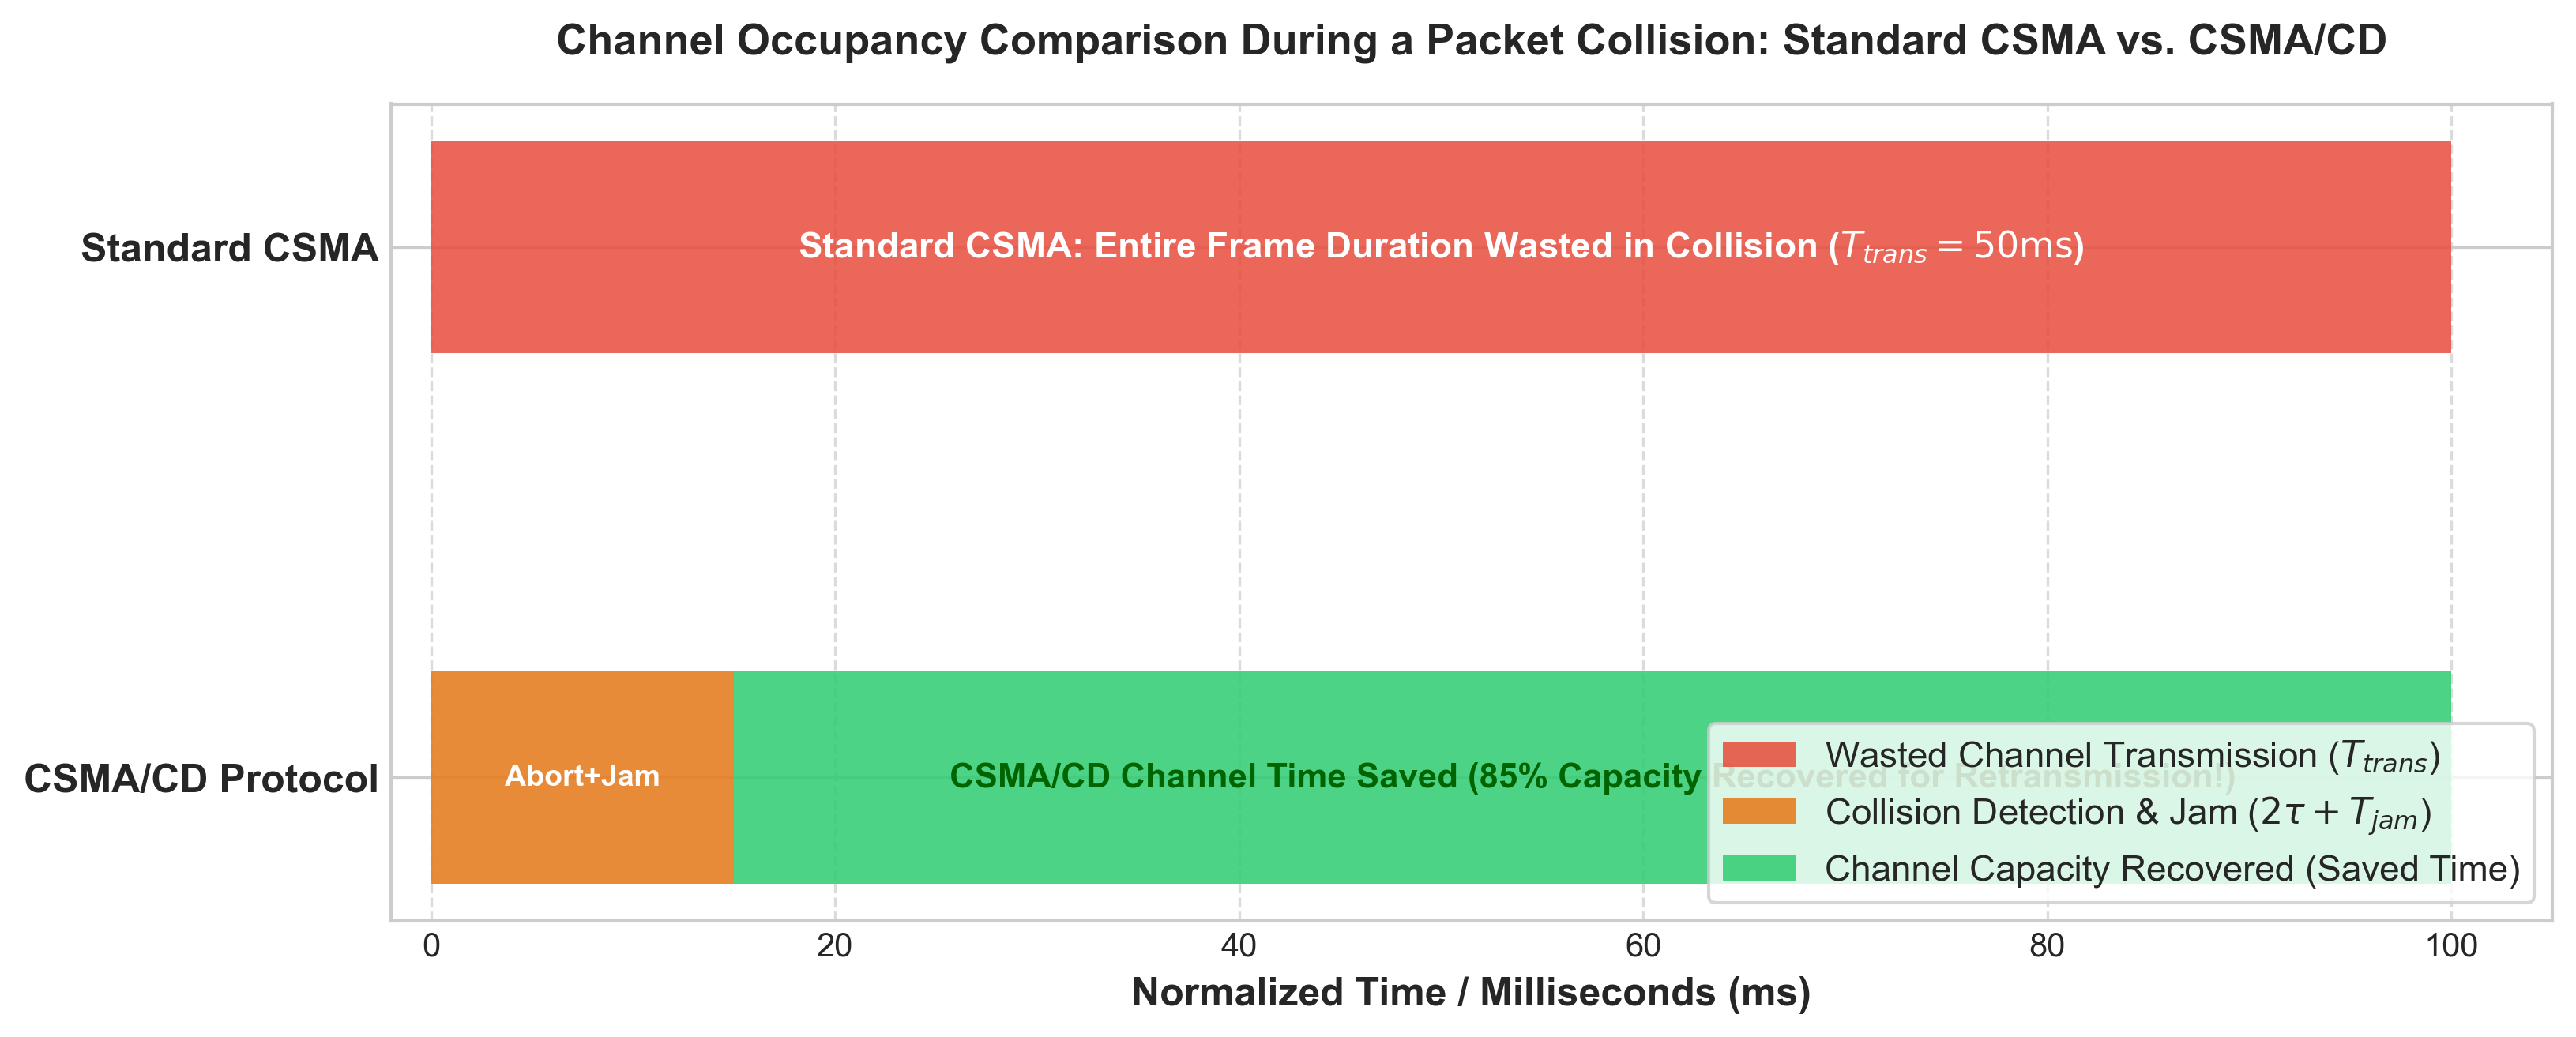
\includegraphics[width=0.9\textwidth]{csma_timeline_diagram.png}
    \caption{Channel Occupancy Comparison During Packet Collision: Standard CSMA vs. CSMA/CD Fast Abort}
    \label{fig:timeline_plot}
\end{figure}

\textbf{Insight from Timeline Analysis:} In standard CSMA (1-Persistent, Non-Persistent, $p$-Persistent), a collision consumes the entire $50\text{ ms}$ transmission window. In CSMA/CD, the collision is detected and jammed within $2\tau + T_{jam} \approx 7.5\text{ ms}$. This immediately liberates the remaining $42.5\text{ ms}$ ($85\%$ of the transmission window), enabling contending stations to back off and re-attempt transmission almost instantaneously. This capacity recovery directly accounts for CSMA/CD's superior throughput and lowest transmission delay across all contention regimes.


% -------------------------------------------------------------
% SECTION 10: COMPARATIVE DISCUSSION
% -------------------------------------------------------------
\section{Comparative Discussion \& Protocol Tradeoffs}

The empirical benchmarks and mathematical derivations in this project demonstrate that no single Medium Access Control protocol is universally superior under all operating conditions. Instead, network designers face complex tradeoffs between \textbf{implementation simplicity, transmission latency, collision frequency, and channel efficiency}.

\subsection{Light Traffic Load Regime ($N \le 2$)}
Under light traffic, the shared medium is idle most of the time.
\begin{itemize}
    \item \textbf{1-Persistent CSMA} is highly competitive, offering near-zero transmission delay because stations transmit immediately upon sensing an idle medium without waiting for backoff timers.
    \item \textbf{Non-Persistent and $p$-Persistent CSMA} suffer from unnecessary latency overhead. Non-persistent stations occasionally defer even when the wire is about to clear, while $p$-persistent stations waste idle slots when $p < 1$.
\end{itemize}

\subsection{Heavy Traffic Load Regime ($N \ge 10$)}
As the number of contending stations escalates, the ranking flips dramatically:
\begin{itemize}
    \item \textbf{1-Persistent CSMA catastrophically collapses.} As seen in Figure \ref{fig:comparison_plot}, throughput plunges below $1\text{ frame/sec}$ and efficiency falls to $2\%$, overwhelmed by repeated collision avalanches.
    \item \textbf{Non-Persistent CSMA} exhibits remarkable resilience, sustaining $44\%$ efficiency at $N = 20$. Its policy of randomized sleep upon sensing busy wire successfully scatters contending stations across time.
    \item \textbf{$p$-Persistent CSMA} maintains steady performance ($50\%$ efficiency) provided $p$ is calibrated dynamically to $\approx 1/N$.
    \item \textbf{CSMA/CD establishes absolute dominance.} By terminating collisions within a fraction of a frame time and dynamically expanding the contention window via Binary Exponential Backoff, CSMA/CD achieves the highest throughput ($11.2\text{ fps}$), highest efficiency ($56\%$), and lowest average delay ($765\text{ ms}$) among all protocols.
\end{itemize}

\subsection{Architectural Legacy of CSMA}
In modern high-speed enterprise networks, half-duplex shared coaxial Ethernet has been replaced by \textbf{Full-Duplex Switched Ethernet (IEEE 802.3u / 802.3ab)}. In switched Ethernet, each station is connected to a dedicated switch port via separate transmit and receive twisted pairs. Because the switch buffers frames and establishes dedicated point-to-point micro-collision domains, packet collisions are physically impossible, and CSMA/CD is disabled in Gigabit+ Ethernet.

Nonetheless, the algorithmic principles engineered in this project remain vital:
\begin{enumerate}
    \item \textbf{Wireless LANs (IEEE 802.11 a/b/g/n/ac/ax):} Wi-Fi networks rely fundamentally on CSMA/CA with exponential backoff contention windows.
    \item \textbf{Industrial Fieldbuses (CAN Bus):} Controller Area Networks in automotive engineering use non-destructive bitwise carrier sensing arbitration.
    \item \textbf{Underwater Acoustic \& Satellite Networks:} High-latency networks continue to utilize variations of slotted $p$-persistent access to optimize channel utilization.
\end{enumerate}


% -------------------------------------------------------------
% SECTION 11: CONCLUSION
% -------------------------------------------------------------
\section{Conclusion}

In this laboratory project, we successfully engineered, implemented, and benchmarked a complete suite of Medium Access Control protocols—\textbf{1-Persistent CSMA, Non-Persistent CSMA, $p$-Persistent CSMA, and CSMA/CD with Truncated Binary Exponential Backoff}—operating over an emulated shared physical channel using POSIX UDP Sockets in C++.

By structuring the channel as an asynchronous event-driven server managing \texttt{IDLE}, \texttt{BUSY}, and \texttt{COLLISION} states with millisecond-precision timers, we observed the true distributed behavior of multi-access channels:
\begin{enumerate}
    \item \textbf{1-Persistent CSMA} provides minimal delay under light traffic but collapses catastrophically under heavy contention due to synchronous collision avalanches.
    \item \textbf{Non-Persistent CSMA} successfully mitigates collisions by enforcing randomized dormancy upon encountering a busy channel, maintaining high stability under heavy load at the expense of slight channel idleness under light traffic.
    \item \textbf{$p$-Persistent CSMA} achieves optimal slotted performance when its parameter is tuned to $p^* \approx 1/N$, empirically confirming classical binomial probability models.
    \item \textbf{CSMA/CD} proves to be the most optimal protocol overall. By enforcing ``Listen While Transmit'' and aborting collisions within $2\tau$, it recovers over $85\%$ of the channel capacity that standard CSMA squanders, while its Truncated Binary Exponential Backoff algorithm dynamically resolves contention ties among dozens of competing stations.
\end{enumerate}

Ultimately, this project bridged the gap between theoretical medium access mathematics and real-world asynchronous socket engineering, providing deep practical insights into how distributed network nodes negotiate shared resources in the physical world.

The complete, multi-process C++ source code, Makefile, Python benchmarking scripts, and generated figures for this project are open-source and available on GitHub at:
\begin{center}
    \url{https://github.com/KaizerEntropy/Computer_Networks_Sem5}
\end{center}

\end{document}
